
\documentclass{article}
%%%%%%%%%%%%%%%%%%%%%%%%%%%%%%%%%%%%%%%%%%%%%%%%%%%%%%%%%%%%%%%%%%%%%%%%%%%%%%%%%%%%%%%%%%%%%%%%%%%%%%%%%%%%%%%%%%%%%%%%%%%%%%%%%%%%%%%%%%%%%%%%%%%%%%%%%%%%%%%%%%%%%%%%%%%%%%%%%%%%%%%%%%%%%%%%%%%%%%%%%%%%%%%%%%%%%%%%%%%%%%%%%%%%%%%%%%%%%%%%%%%%%%%%%%%%
\usepackage{amssymb}
\usepackage{amsfonts}
\usepackage{amsmath}
\usepackage{graphicx}
\usepackage{float}
\usepackage{caption}
\usepackage{booktabs}

\setcounter{MaxMatrixCols}{10}
%TCIDATA{OutputFilter=LATEX.DLL}
%TCIDATA{Version=5.50.0.2953}
%TCIDATA{<META NAME="SaveForMode" CONTENT="1">}
%TCIDATA{BibliographyScheme=Manual}
%TCIDATA{Created=Tuesday, February 04, 2020 09:00:51}
%TCIDATA{LastRevised=Wednesday, May 20, 2020 21:49:55}
%TCIDATA{<META NAME="GraphicsSave" CONTENT="32">}
%TCIDATA{<META NAME="DocumentShell" CONTENT="Standard LaTeX\Standard LaTeX Article">}
%TCIDATA{Language=American English}
%TCIDATA{CSTFile=40 LaTeX article.cst}

\newtheorem{theorem}{Theorem}
\newtheorem{acknowledgment}[theorem]{Acknowledgment}
\newtheorem{algorithm}[theorem]{Algorithm}
\newtheorem{axiom}[theorem]{Axiom}
\newtheorem{case}[theorem]{Case}
\newtheorem{claim}[theorem]{Claim}
\newtheorem{conclusion}[theorem]{Conclusion}
\newtheorem{condition}[theorem]{Condition}
\newtheorem{conjecture}[theorem]{Conjecture}
\newtheorem{corollary}[theorem]{Corollary}
\newtheorem{criterion}[theorem]{Criterion}
\newtheorem{definition}[theorem]{Definition}
\newtheorem{example}[theorem]{Example}
\newtheorem{exercise}[theorem]{Exercise}
\newtheorem{lemma}[theorem]{Lemma}
\newtheorem{notation}[theorem]{Notation}
\newtheorem{problem}[theorem]{Problem}
\newtheorem{proposition}[theorem]{Proposition}
\newtheorem{remark}[theorem]{Remark}
\newtheorem{solution}[theorem]{Solution}
\newtheorem{summary}[theorem]{Summary}
\newenvironment{proof}[1][Proof]{\noindent\textbf{#1.} }{\ \rule{0.5em}{0.5em}}
% Macros for Scientific Word and Scientific WorkPlace 5.5 documents saved with the LaTeX filter.
% Copyright (C) 2005 Mackichan Software, Inc.

\typeout{TCILATEX Macros for Scientific Word and Scientific WorkPlace 5.5 <06 Oct 2005>.}
\typeout{NOTICE:  This macro file is NOT proprietary and may be 
freely copied and distributed.}
%
\makeatletter

%%%%%%%%%%%%%%%%%%%%%
% pdfTeX related.
\ifx\pdfoutput\relax\let\pdfoutput=\undefined\fi
\newcount\msipdfoutput
\ifx\pdfoutput\undefined
\else
 \ifcase\pdfoutput
 \else 
    \msipdfoutput=1
    \ifx\paperwidth\undefined
    \else
      \ifdim\paperheight=0pt\relax
      \else
        \pdfpageheight\paperheight
      \fi
      \ifdim\paperwidth=0pt\relax
      \else
        \pdfpagewidth\paperwidth
      \fi
    \fi
  \fi  
\fi

%%%%%%%%%%%%%%%%%%%%%
% FMTeXButton
% This is used for putting TeXButtons in the 
% frontmatter of a document. Add a line like
% \QTagDef{FMTeXButton}{101}{} to the filter 
% section of the cst being used. Also add a
% new section containing:
%     [f_101]
%     ALIAS=FMTexButton
%     TAG_TYPE=FIELD
%     TAG_LEADIN=TeX Button:
%
% It also works to put \defs in the preamble after 
% the \input tcilatex
\def\FMTeXButton#1{#1}
%
%%%%%%%%%%%%%%%%%%%%%%
% macros for time
\newcount\@hour\newcount\@minute\chardef\@x10\chardef\@xv60
\def\tcitime{
\def\@time{%
  \@minute\time\@hour\@minute\divide\@hour\@xv
  \ifnum\@hour<\@x 0\fi\the\@hour:%
  \multiply\@hour\@xv\advance\@minute-\@hour
  \ifnum\@minute<\@x 0\fi\the\@minute
  }}%

%%%%%%%%%%%%%%%%%%%%%%
% macro for hyperref and msihyperref
%\@ifundefined{hyperref}{\def\hyperref#1#2#3#4{#2\ref{#4}#3}}{}

\def\x@hyperref#1#2#3{%
   % Turn off various catcodes before reading parameter 4
   \catcode`\~ = 12
   \catcode`\$ = 12
   \catcode`\_ = 12
   \catcode`\# = 12
   \catcode`\& = 12
   \catcode`\% = 12
   \y@hyperref{#1}{#2}{#3}%
}

\def\y@hyperref#1#2#3#4{%
   #2\ref{#4}#3
   \catcode`\~ = 13
   \catcode`\$ = 3
   \catcode`\_ = 8
   \catcode`\# = 6
   \catcode`\& = 4
   \catcode`\% = 14
}

\@ifundefined{hyperref}{\let\hyperref\x@hyperref}{}
\@ifundefined{msihyperref}{\let\msihyperref\x@hyperref}{}




% macro for external program call
\@ifundefined{qExtProgCall}{\def\qExtProgCall#1#2#3#4#5#6{\relax}}{}
%%%%%%%%%%%%%%%%%%%%%%
%
% macros for graphics
%
\def\FILENAME#1{#1}%
%
\def\QCTOpt[#1]#2{%
  \def\QCTOptB{#1}
  \def\QCTOptA{#2}
}
\def\QCTNOpt#1{%
  \def\QCTOptA{#1}
  \let\QCTOptB\empty
}
\def\Qct{%
  \@ifnextchar[{%
    \QCTOpt}{\QCTNOpt}
}
\def\QCBOpt[#1]#2{%
  \def\QCBOptB{#1}%
  \def\QCBOptA{#2}%
}
\def\QCBNOpt#1{%
  \def\QCBOptA{#1}%
  \let\QCBOptB\empty
}
\def\Qcb{%
  \@ifnextchar[{%
    \QCBOpt}{\QCBNOpt}%
}
\def\PrepCapArgs{%
  \ifx\QCBOptA\empty
    \ifx\QCTOptA\empty
      {}%
    \else
      \ifx\QCTOptB\empty
        {\QCTOptA}%
      \else
        [\QCTOptB]{\QCTOptA}%
      \fi
    \fi
  \else
    \ifx\QCBOptA\empty
      {}%
    \else
      \ifx\QCBOptB\empty
        {\QCBOptA}%
      \else
        [\QCBOptB]{\QCBOptA}%
      \fi
    \fi
  \fi
}
\newcount\GRAPHICSTYPE
%\GRAPHICSTYPE 0 is for TurboTeX
%\GRAPHICSTYPE 1 is for DVIWindo (PostScript)
%%%(removed)%\GRAPHICSTYPE 2 is for psfig (PostScript)
\GRAPHICSTYPE=\z@
\def\GRAPHICSPS#1{%
 \ifcase\GRAPHICSTYPE%\GRAPHICSTYPE=0
   \special{ps: #1}%
 \or%\GRAPHICSTYPE=1
   \special{language "PS", include "#1"}%
%%%\or%\GRAPHICSTYPE=2
%%%  #1%
 \fi
}%
%
\def\GRAPHICSHP#1{\special{include #1}}%
%
% \graffile{ body }                                  %#1
%          { contentswidth (scalar)  }               %#2
%          { contentsheight (scalar) }               %#3
%          { vertical shift when in-line (scalar) }  %#4

\def\graffile#1#2#3#4{%
%%% \ifnum\GRAPHICSTYPE=\tw@
%%%  %Following if using psfig
%%%  \@ifundefined{psfig}{\input psfig.tex}{}%
%%%  \psfig{file=#1, height=#3, width=#2}%
%%% \else
  %Following for all others
  % JCS - added BOXTHEFRAME, see below
    \bgroup
	   \@inlabelfalse
       \leavevmode
       \@ifundefined{bbl@deactivate}{\def~{\string~}}{\activesoff}%
        \raise -#4 \BOXTHEFRAME{%
           \hbox to #2{\raise #3\hbox to #2{\null #1\hfil}}}%
    \egroup
}%
%
% A box for drafts
\def\draftbox#1#2#3#4{%
 \leavevmode\raise -#4 \hbox{%
  \frame{\rlap{\protect\tiny #1}\hbox to #2%
   {\vrule height#3 width\z@ depth\z@\hfil}%
  }%
 }%
}%
%
\newcount\@msidraft
\@msidraft=\z@
\let\nographics=\@msidraft
\newif\ifwasdraft
\wasdraftfalse

%  \GRAPHIC{ body }                                  %#1
%          { draft name }                            %#2
%          { contentswidth (scalar)  }               %#3
%          { contentsheight (scalar) }               %#4
%          { vertical shift when in-line (scalar) }  %#5
\def\GRAPHIC#1#2#3#4#5{%
   \ifnum\@msidraft=\@ne\draftbox{#2}{#3}{#4}{#5}%
   \else\graffile{#1}{#3}{#4}{#5}%
   \fi
}
%
\def\addtoLaTeXparams#1{%
    \edef\LaTeXparams{\LaTeXparams #1}}%
%
% JCS -  added a switch BoxFrame that can 
% be set by including X in the frame params.
% If set a box is drawn around the frame.

\newif\ifBoxFrame \BoxFramefalse
\newif\ifOverFrame \OverFramefalse
\newif\ifUnderFrame \UnderFramefalse

\def\BOXTHEFRAME#1{%
   \hbox{%
      \ifBoxFrame
         \frame{#1}%
      \else
         {#1}%
      \fi
   }%
}


\def\doFRAMEparams#1{\BoxFramefalse\OverFramefalse\UnderFramefalse\readFRAMEparams#1\end}%
\def\readFRAMEparams#1{%
 \ifx#1\end%
  \let\next=\relax
  \else
  \ifx#1i\dispkind=\z@\fi
  \ifx#1d\dispkind=\@ne\fi
  \ifx#1f\dispkind=\tw@\fi
  \ifx#1t\addtoLaTeXparams{t}\fi
  \ifx#1b\addtoLaTeXparams{b}\fi
  \ifx#1p\addtoLaTeXparams{p}\fi
  \ifx#1h\addtoLaTeXparams{h}\fi
  \ifx#1X\BoxFrametrue\fi
  \ifx#1O\OverFrametrue\fi
  \ifx#1U\UnderFrametrue\fi
  \ifx#1w
    \ifnum\@msidraft=1\wasdrafttrue\else\wasdraftfalse\fi
    \@msidraft=\@ne
  \fi
  \let\next=\readFRAMEparams
  \fi
 \next
 }%
%
%Macro for In-line graphics object
%   \IFRAME{ contentswidth (scalar)  }               %#1
%          { contentsheight (scalar) }               %#2
%          { vertical shift when in-line (scalar) }  %#3
%          { draft name }                            %#4
%          { body }                                  %#5
%          { caption}                                %#6


\def\IFRAME#1#2#3#4#5#6{%
      \bgroup
      \let\QCTOptA\empty
      \let\QCTOptB\empty
      \let\QCBOptA\empty
      \let\QCBOptB\empty
      #6%
      \parindent=0pt
      \leftskip=0pt
      \rightskip=0pt
      \setbox0=\hbox{\QCBOptA}%
      \@tempdima=#1\relax
      \ifOverFrame
          % Do this later
          \typeout{This is not implemented yet}%
          \show\HELP
      \else
         \ifdim\wd0>\@tempdima
            \advance\@tempdima by \@tempdima
            \ifdim\wd0 >\@tempdima
               \setbox1 =\vbox{%
                  \unskip\hbox to \@tempdima{\hfill\GRAPHIC{#5}{#4}{#1}{#2}{#3}\hfill}%
                  \unskip\hbox to \@tempdima{\parbox[b]{\@tempdima}{\QCBOptA}}%
               }%
               \wd1=\@tempdima
            \else
               \textwidth=\wd0
               \setbox1 =\vbox{%
                 \noindent\hbox to \wd0{\hfill\GRAPHIC{#5}{#4}{#1}{#2}{#3}\hfill}\\%
                 \noindent\hbox{\QCBOptA}%
               }%
               \wd1=\wd0
            \fi
         \else
            \ifdim\wd0>0pt
              \hsize=\@tempdima
              \setbox1=\vbox{%
                \unskip\GRAPHIC{#5}{#4}{#1}{#2}{0pt}%
                \break
                \unskip\hbox to \@tempdima{\hfill \QCBOptA\hfill}%
              }%
              \wd1=\@tempdima
           \else
              \hsize=\@tempdima
              \setbox1=\vbox{%
                \unskip\GRAPHIC{#5}{#4}{#1}{#2}{0pt}%
              }%
              \wd1=\@tempdima
           \fi
         \fi
         \@tempdimb=\ht1
         %\advance\@tempdimb by \dp1
         \advance\@tempdimb by -#2
         \advance\@tempdimb by #3
         \leavevmode
         \raise -\@tempdimb \hbox{\box1}%
      \fi
      \egroup%
}%
%
%Macro for Display graphics object
%   \DFRAME{ contentswidth (scalar)  }               %#1
%          { contentsheight (scalar) }               %#2
%          { draft label }                           %#3
%          { name }                                  %#4
%          { caption}                                %#5
\def\DFRAME#1#2#3#4#5{%
  \vspace\topsep
  \hfil\break
  \bgroup
     \leftskip\@flushglue
	 \rightskip\@flushglue
	 \parindent\z@
	 \parfillskip\z@skip
     \let\QCTOptA\empty
     \let\QCTOptB\empty
     \let\QCBOptA\empty
     \let\QCBOptB\empty
	 \vbox\bgroup
        \ifOverFrame 
           #5\QCTOptA\par
        \fi
        \GRAPHIC{#4}{#3}{#1}{#2}{\z@}%
        \ifUnderFrame 
           \break#5\QCBOptA
        \fi
	 \egroup
  \egroup
  \vspace\topsep
  \break
}%
%
%Macro for Floating graphic object
%   \FFRAME{ framedata f|i tbph x F|T }              %#1
%          { contentswidth (scalar)  }               %#2
%          { contentsheight (scalar) }               %#3
%          { caption }                               %#4
%          { label }                                 %#5
%          { draft name }                            %#6
%          { body }                                  %#7
\def\FFRAME#1#2#3#4#5#6#7{%
 %If float.sty loaded and float option is 'h', change to 'H'  (gp) 1998/09/05
  \@ifundefined{floatstyle}
    {%floatstyle undefined (and float.sty not present), no change
     \begin{figure}[#1]%
    }
    {%floatstyle DEFINED
	 \ifx#1h%Only the h parameter, change to H
      \begin{figure}[H]%
	 \else
      \begin{figure}[#1]%
	 \fi
	}
  \let\QCTOptA\empty
  \let\QCTOptB\empty
  \let\QCBOptA\empty
  \let\QCBOptB\empty
  \ifOverFrame
    #4
    \ifx\QCTOptA\empty
    \else
      \ifx\QCTOptB\empty
        \caption{\QCTOptA}%
      \else
        \caption[\QCTOptB]{\QCTOptA}%
      \fi
    \fi
    \ifUnderFrame\else
      \label{#5}%
    \fi
  \else
    \UnderFrametrue%
  \fi
  \begin{center}\GRAPHIC{#7}{#6}{#2}{#3}{\z@}\end{center}%
  \ifUnderFrame
    #4
    \ifx\QCBOptA\empty
      \caption{}%
    \else
      \ifx\QCBOptB\empty
        \caption{\QCBOptA}%
      \else
        \caption[\QCBOptB]{\QCBOptA}%
      \fi
    \fi
    \label{#5}%
  \fi
  \end{figure}%
 }%
%
%
%    \FRAME{ framedata f|i tbph x F|T }              %#1
%          { contentswidth (scalar)  }               %#2
%          { contentsheight (scalar) }               %#3
%          { vertical shift when in-line (scalar) }  %#4
%          { caption }                               %#5
%          { label }                                 %#6
%          { name }                                  %#7
%          { body }                                  %#8
%
%    framedata is a string which can contain the following
%    characters: idftbphxFT
%    Their meaning is as follows:
%             i, d or f : in-line, display, or floating
%             t,b,p,h   : LaTeX floating placement options
%             x         : fit contents box to contents
%             F or T    : Figure or Table. 
%                         Later this can expand
%                         to a more general float class.
%
%
\newcount\dispkind%

\def\makeactives{
  \catcode`\"=\active
  \catcode`\;=\active
  \catcode`\:=\active
  \catcode`\'=\active
  \catcode`\~=\active
}
\bgroup
   \makeactives
   \gdef\activesoff{%
      \def"{\string"}%
      \def;{\string;}%
      \def:{\string:}%
      \def'{\string'}%
      \def~{\string~}%
      %\bbl@deactivate{"}%
      %\bbl@deactivate{;}%
      %\bbl@deactivate{:}%
      %\bbl@deactivate{'}%
    }
\egroup

\def\FRAME#1#2#3#4#5#6#7#8{%
 \bgroup
 \ifnum\@msidraft=\@ne
   \wasdrafttrue
 \else
   \wasdraftfalse%
 \fi
 \def\LaTeXparams{}%
 \dispkind=\z@
 \def\LaTeXparams{}%
 \doFRAMEparams{#1}%
 \ifnum\dispkind=\z@\IFRAME{#2}{#3}{#4}{#7}{#8}{#5}\else
  \ifnum\dispkind=\@ne\DFRAME{#2}{#3}{#7}{#8}{#5}\else
   \ifnum\dispkind=\tw@
    \edef\@tempa{\noexpand\FFRAME{\LaTeXparams}}%
    \@tempa{#2}{#3}{#5}{#6}{#7}{#8}%
    \fi
   \fi
  \fi
  \ifwasdraft\@msidraft=1\else\@msidraft=0\fi{}%
  \egroup
 }%
%
% This macro added to let SW gobble a parameter that
% should not be passed on and expanded. 

\def\TEXUX#1{"texux"}

%
% Macros for text attributes:
%
\def\BF#1{{\bf {#1}}}%
\def\NEG#1{\leavevmode\hbox{\rlap{\thinspace/}{$#1$}}}%
%
%%%%%%%%%%%%%%%%%%%%%%%%%%%%%%%%%%%%%%%%%%%%%%%%%%%%%%%%%%%%%%%%%%%%%%%%
%
%
% macros for user - defined functions
\def\limfunc#1{\mathop{\rm #1}}%
\def\func#1{\mathop{\rm #1}\nolimits}%
% macro for unit names
\def\unit#1{\mathord{\thinspace\rm #1}}%

%
% miscellaneous 
\long\def\QQQ#1#2{%
     \long\expandafter\def\csname#1\endcsname{#2}}%
\@ifundefined{QTP}{\def\QTP#1{}}{}
\@ifundefined{QEXCLUDE}{\def\QEXCLUDE#1{}}{}
\@ifundefined{Qlb}{\def\Qlb#1{#1}}{}
\@ifundefined{Qlt}{\def\Qlt#1{#1}}{}
\def\QWE{}%
\long\def\QQA#1#2{}%
\def\QTR#1#2{{\csname#1\endcsname {#2}}}%
  %	Add aliases for the ulem package
  \let\QQQuline\uline
  \let\QQQsout\sout
  \let\QQQuuline\uuline
  \let\QQQuwave\uwave
  \let\QQQxout\xout
\long\def\TeXButton#1#2{#2}%
\long\def\QSubDoc#1#2{#2}%
\def\EXPAND#1[#2]#3{}%
\def\NOEXPAND#1[#2]#3{}%
\def\PROTECTED{}%
\def\LaTeXparent#1{}%
\def\ChildStyles#1{}%
\def\ChildDefaults#1{}%
\def\QTagDef#1#2#3{}%

% Constructs added with Scientific Notebook
\@ifundefined{correctchoice}{\def\correctchoice{\relax}}{}
\@ifundefined{HTML}{\def\HTML#1{\relax}}{}
\@ifundefined{TCIIcon}{\def\TCIIcon#1#2#3#4{\relax}}{}
\if@compatibility
  \typeout{Not defining UNICODE  U or CustomNote commands for LaTeX 2.09.}
\else
  \providecommand{\UNICODE}[2][]{\protect\rule{.1in}{.1in}}
  \providecommand{\U}[1]{\protect\rule{.1in}{.1in}}
  \providecommand{\CustomNote}[3][]{\marginpar{#3}}
\fi

\@ifundefined{lambdabar}{
      \def\lambdabar{\errmessage{You have used the lambdabar symbol. 
                      This is available for typesetting only in RevTeX styles.}}
   }{}

%
% Macros for style editor docs
\@ifundefined{StyleEditBeginDoc}{\def\StyleEditBeginDoc{\relax}}{}
%
% Macros for footnotes
\def\QQfnmark#1{\footnotemark}
\def\QQfntext#1#2{\addtocounter{footnote}{#1}\footnotetext{#2}}
%
% Macros for indexing.
%
\@ifundefined{TCIMAKEINDEX}{}{\makeindex}%
%
% Attempts to avoid problems with other styles
\@ifundefined{abstract}{%
 \def\abstract{%
  \if@twocolumn
   \section*{Abstract (Not appropriate in this style!)}%
   \else \small 
   \begin{center}{\bf Abstract\vspace{-.5em}\vspace{\z@}}\end{center}%
   \quotation 
   \fi
  }%
 }{%
 }%
\@ifundefined{endabstract}{\def\endabstract
  {\if@twocolumn\else\endquotation\fi}}{}%
\@ifundefined{maketitle}{\def\maketitle#1{}}{}%
\@ifundefined{affiliation}{\def\affiliation#1{}}{}%
\@ifundefined{proof}{\def\proof{\noindent{\bfseries Proof. }}}{}%
\@ifundefined{endproof}{\def\endproof{\mbox{\ \rule{.1in}{.1in}}}}{}%
\@ifundefined{newfield}{\def\newfield#1#2{}}{}%
\@ifundefined{chapter}{\def\chapter#1{\par(Chapter head:)#1\par }%
 \newcount\c@chapter}{}%
\@ifundefined{part}{\def\part#1{\par(Part head:)#1\par }}{}%
\@ifundefined{section}{\def\section#1{\par(Section head:)#1\par }}{}%
\@ifundefined{subsection}{\def\subsection#1%
 {\par(Subsection head:)#1\par }}{}%
\@ifundefined{subsubsection}{\def\subsubsection#1%
 {\par(Subsubsection head:)#1\par }}{}%
\@ifundefined{paragraph}{\def\paragraph#1%
 {\par(Subsubsubsection head:)#1\par }}{}%
\@ifundefined{subparagraph}{\def\subparagraph#1%
 {\par(Subsubsubsubsection head:)#1\par }}{}%
%%%%%%%%%%%%%%%%%%%%%%%%%%%%%%%%%%%%%%%%%%%%%%%%%%%%%%%%%%%%%%%%%%%%%%%%
% These symbols are not recognized by LaTeX
\@ifundefined{therefore}{\def\therefore{}}{}%
\@ifundefined{backepsilon}{\def\backepsilon{}}{}%
\@ifundefined{yen}{\def\yen{\hbox{\rm\rlap=Y}}}{}%
\@ifundefined{registered}{%
   \def\registered{\relax\ifmmode{}\r@gistered
                    \else$\m@th\r@gistered$\fi}%
 \def\r@gistered{^{\ooalign
  {\hfil\raise.07ex\hbox{$\scriptstyle\rm\text{R}$}\hfil\crcr
  \mathhexbox20D}}}}{}%
\@ifundefined{Eth}{\def\Eth{}}{}%
\@ifundefined{eth}{\def\eth{}}{}%
\@ifundefined{Thorn}{\def\Thorn{}}{}%
\@ifundefined{thorn}{\def\thorn{}}{}%
% A macro to allow any symbol that requires math to appear in text
\def\TEXTsymbol#1{\mbox{$#1$}}%
\@ifundefined{degree}{\def\degree{{}^{\circ}}}{}%
%
% macros for T3TeX files
\newdimen\theight
\@ifundefined{Column}{\def\Column{%
 \vadjust{\setbox\z@=\hbox{\scriptsize\quad\quad tcol}%
  \theight=\ht\z@\advance\theight by \dp\z@\advance\theight by \lineskip
  \kern -\theight \vbox to \theight{%
   \rightline{\rlap{\box\z@}}%
   \vss
   }%
  }%
 }}{}%
%
\@ifundefined{qed}{\def\qed{%
 \ifhmode\unskip\nobreak\fi\ifmmode\ifinner\else\hskip5\p@\fi\fi
 \hbox{\hskip5\p@\vrule width4\p@ height6\p@ depth1.5\p@\hskip\p@}%
 }}{}%
%
\@ifundefined{cents}{\def\cents{\hbox{\rm\rlap c/}}}{}%
\@ifundefined{tciLaplace}{\def\tciLaplace{\ensuremath{\mathcal{L}}}}{}%
\@ifundefined{tciFourier}{\def\tciFourier{\ensuremath{\mathcal{F}}}}{}%
\@ifundefined{textcurrency}{\def\textcurrency{\hbox{\rm\rlap xo}}}{}%
\@ifundefined{texteuro}{\def\texteuro{\hbox{\rm\rlap C=}}}{}%
\@ifundefined{euro}{\def\euro{\hbox{\rm\rlap C=}}}{}%
\@ifundefined{textfranc}{\def\textfranc{\hbox{\rm\rlap-F}}}{}%
\@ifundefined{textlira}{\def\textlira{\hbox{\rm\rlap L=}}}{}%
\@ifundefined{textpeseta}{\def\textpeseta{\hbox{\rm P\negthinspace s}}}{}%
%
\@ifundefined{miss}{\def\miss{\hbox{\vrule height2\p@ width 2\p@ depth\z@}}}{}%
%
\@ifundefined{vvert}{\def\vvert{\Vert}}{}%  %always translated to \left| or \right|
%
\@ifundefined{tcol}{\def\tcol#1{{\baselineskip=6\p@ \vcenter{#1}} \Column}}{}%
%
\@ifundefined{dB}{\def\dB{\hbox{{}}}}{}%        %dummy entry in column 
\@ifundefined{mB}{\def\mB#1{\hbox{$#1$}}}{}%   %column entry
\@ifundefined{nB}{\def\nB#1{\hbox{#1}}}{}%     %column entry (not math)
%
\@ifundefined{note}{\def\note{$^{\dag}}}{}%
%
\def\newfmtname{LaTeX2e}
% No longer load latexsym.  This is now handled by SWP, which uses amsfonts if necessary
%
\ifx\fmtname\newfmtname
  \DeclareOldFontCommand{\rm}{\normalfont\rmfamily}{\mathrm}
  \DeclareOldFontCommand{\sf}{\normalfont\sffamily}{\mathsf}
  \DeclareOldFontCommand{\tt}{\normalfont\ttfamily}{\mathtt}
  \DeclareOldFontCommand{\bf}{\normalfont\bfseries}{\mathbf}
  \DeclareOldFontCommand{\it}{\normalfont\itshape}{\mathit}
  \DeclareOldFontCommand{\sl}{\normalfont\slshape}{\@nomath\sl}
  \DeclareOldFontCommand{\sc}{\normalfont\scshape}{\@nomath\sc}
\fi

%
% Greek bold macros
% Redefine all of the math symbols 
% which might be bolded	 - there are 
% probably others to add to this list

\def\alpha{{\Greekmath 010B}}%
\def\beta{{\Greekmath 010C}}%
\def\gamma{{\Greekmath 010D}}%
\def\delta{{\Greekmath 010E}}%
\def\epsilon{{\Greekmath 010F}}%
\def\zeta{{\Greekmath 0110}}%
\def\eta{{\Greekmath 0111}}%
\def\theta{{\Greekmath 0112}}%
\def\iota{{\Greekmath 0113}}%
\def\kappa{{\Greekmath 0114}}%
\def\lambda{{\Greekmath 0115}}%
\def\mu{{\Greekmath 0116}}%
\def\nu{{\Greekmath 0117}}%
\def\xi{{\Greekmath 0118}}%
\def\pi{{\Greekmath 0119}}%
\def\rho{{\Greekmath 011A}}%
\def\sigma{{\Greekmath 011B}}%
\def\tau{{\Greekmath 011C}}%
\def\upsilon{{\Greekmath 011D}}%
\def\phi{{\Greekmath 011E}}%
\def\chi{{\Greekmath 011F}}%
\def\psi{{\Greekmath 0120}}%
\def\omega{{\Greekmath 0121}}%
\def\varepsilon{{\Greekmath 0122}}%
\def\vartheta{{\Greekmath 0123}}%
\def\varpi{{\Greekmath 0124}}%
\def\varrho{{\Greekmath 0125}}%
\def\varsigma{{\Greekmath 0126}}%
\def\varphi{{\Greekmath 0127}}%

\def\nabla{{\Greekmath 0272}}
\def\FindBoldGroup{%
   {\setbox0=\hbox{$\mathbf{x\global\edef\theboldgroup{\the\mathgroup}}$}}%
}

\def\Greekmath#1#2#3#4{%
    \if@compatibility
        \ifnum\mathgroup=\symbold
           \mathchoice{\mbox{\boldmath$\displaystyle\mathchar"#1#2#3#4$}}%
                      {\mbox{\boldmath$\textstyle\mathchar"#1#2#3#4$}}%
                      {\mbox{\boldmath$\scriptstyle\mathchar"#1#2#3#4$}}%
                      {\mbox{\boldmath$\scriptscriptstyle\mathchar"#1#2#3#4$}}%
        \else
           \mathchar"#1#2#3#4% 
        \fi 
    \else 
        \FindBoldGroup
        \ifnum\mathgroup=\theboldgroup % For 2e
           \mathchoice{\mbox{\boldmath$\displaystyle\mathchar"#1#2#3#4$}}%
                      {\mbox{\boldmath$\textstyle\mathchar"#1#2#3#4$}}%
                      {\mbox{\boldmath$\scriptstyle\mathchar"#1#2#3#4$}}%
                      {\mbox{\boldmath$\scriptscriptstyle\mathchar"#1#2#3#4$}}%
        \else
           \mathchar"#1#2#3#4% 
        \fi     	    
	  \fi}

\newif\ifGreekBold  \GreekBoldfalse
\let\SAVEPBF=\pbf
\def\pbf{\GreekBoldtrue\SAVEPBF}%
%

\@ifundefined{theorem}{\newtheorem{theorem}{Theorem}}{}
\@ifundefined{lemma}{\newtheorem{lemma}[theorem]{Lemma}}{}
\@ifundefined{corollary}{\newtheorem{corollary}[theorem]{Corollary}}{}
\@ifundefined{conjecture}{\newtheorem{conjecture}[theorem]{Conjecture}}{}
\@ifundefined{proposition}{\newtheorem{proposition}[theorem]{Proposition}}{}
\@ifundefined{axiom}{\newtheorem{axiom}{Axiom}}{}
\@ifundefined{remark}{\newtheorem{remark}{Remark}}{}
\@ifundefined{example}{\newtheorem{example}{Example}}{}
\@ifundefined{exercise}{\newtheorem{exercise}{Exercise}}{}
\@ifundefined{definition}{\newtheorem{definition}{Definition}}{}


\@ifundefined{mathletters}{%
  %\def\theequation{\arabic{equation}}
  \newcounter{equationnumber}  
  \def\mathletters{%
     \addtocounter{equation}{1}
     \edef\@currentlabel{\theequation}%
     \setcounter{equationnumber}{\c@equation}
     \setcounter{equation}{0}%
     \edef\theequation{\@currentlabel\noexpand\alph{equation}}%
  }
  \def\endmathletters{%
     \setcounter{equation}{\value{equationnumber}}%
  }
}{}

%Logos
\@ifundefined{BibTeX}{%
    \def\BibTeX{{\rm B\kern-.05em{\sc i\kern-.025em b}\kern-.08em
                 T\kern-.1667em\lower.7ex\hbox{E}\kern-.125emX}}}{}%
\@ifundefined{AmS}%
    {\def\AmS{{\protect\usefont{OMS}{cmsy}{m}{n}%
                A\kern-.1667em\lower.5ex\hbox{M}\kern-.125emS}}}{}%
\@ifundefined{AmSTeX}{\def\AmSTeX{\protect\AmS-\protect\TeX\@}}{}%
%

% This macro is a fix to eqnarray
\def\@@eqncr{\let\@tempa\relax
    \ifcase\@eqcnt \def\@tempa{& & &}\or \def\@tempa{& &}%
      \else \def\@tempa{&}\fi
     \@tempa
     \if@eqnsw
        \iftag@
           \@taggnum
        \else
           \@eqnnum\stepcounter{equation}%
        \fi
     \fi
     \global\tag@false
     \global\@eqnswtrue
     \global\@eqcnt\z@\cr}


\def\TCItag{\@ifnextchar*{\@TCItagstar}{\@TCItag}}
\def\@TCItag#1{%
    \global\tag@true
    \global\def\@taggnum{(#1)}%
    \global\def\@currentlabel{#1}}
\def\@TCItagstar*#1{%
    \global\tag@true
    \global\def\@taggnum{#1}%
    \global\def\@currentlabel{#1}}
%
%%%%%%%%%%%%%%%%%%%%%%%%%%%%%%%%%%%%%%%%%%%%%%%%%%%%%%%%%%%%%%%%%%%%%
%
\def\QATOP#1#2{{#1 \atop #2}}%
\def\QTATOP#1#2{{\textstyle {#1 \atop #2}}}%
\def\QDATOP#1#2{{\displaystyle {#1 \atop #2}}}%
\def\QABOVE#1#2#3{{#2 \above#1 #3}}%
\def\QTABOVE#1#2#3{{\textstyle {#2 \above#1 #3}}}%
\def\QDABOVE#1#2#3{{\displaystyle {#2 \above#1 #3}}}%
\def\QOVERD#1#2#3#4{{#3 \overwithdelims#1#2 #4}}%
\def\QTOVERD#1#2#3#4{{\textstyle {#3 \overwithdelims#1#2 #4}}}%
\def\QDOVERD#1#2#3#4{{\displaystyle {#3 \overwithdelims#1#2 #4}}}%
\def\QATOPD#1#2#3#4{{#3 \atopwithdelims#1#2 #4}}%
\def\QTATOPD#1#2#3#4{{\textstyle {#3 \atopwithdelims#1#2 #4}}}%
\def\QDATOPD#1#2#3#4{{\displaystyle {#3 \atopwithdelims#1#2 #4}}}%
\def\QABOVED#1#2#3#4#5{{#4 \abovewithdelims#1#2#3 #5}}%
\def\QTABOVED#1#2#3#4#5{{\textstyle 
   {#4 \abovewithdelims#1#2#3 #5}}}%
\def\QDABOVED#1#2#3#4#5{{\displaystyle 
   {#4 \abovewithdelims#1#2#3 #5}}}%
%
% Macros for text size operators:
%

\def\tint{\msi@int\textstyle\int}%
\def\tiint{\msi@int\textstyle\iint}%
\def\tiiint{\msi@int\textstyle\iiint}%
\def\tiiiint{\msi@int\textstyle\iiiint}%
\def\tidotsint{\msi@int\textstyle\idotsint}%
\def\toint{\msi@int\textstyle\oint}%


\def\tsum{\mathop{\textstyle \sum }}%
\def\tprod{\mathop{\textstyle \prod }}%
\def\tbigcap{\mathop{\textstyle \bigcap }}%
\def\tbigwedge{\mathop{\textstyle \bigwedge }}%
\def\tbigoplus{\mathop{\textstyle \bigoplus }}%
\def\tbigodot{\mathop{\textstyle \bigodot }}%
\def\tbigsqcup{\mathop{\textstyle \bigsqcup }}%
\def\tcoprod{\mathop{\textstyle \coprod }}%
\def\tbigcup{\mathop{\textstyle \bigcup }}%
\def\tbigvee{\mathop{\textstyle \bigvee }}%
\def\tbigotimes{\mathop{\textstyle \bigotimes }}%
\def\tbiguplus{\mathop{\textstyle \biguplus }}%
%
%
%Macros for display size operators:
%

\newtoks\temptoksa
\newtoks\temptoksb
\newtoks\temptoksc


\def\msi@int#1#2{%
 \def\@temp{{#1#2\the\temptoksc_{\the\temptoksa}^{\the\temptoksb}}}%   
 \futurelet\@nextcs
 \@int
}

\def\@int{%
   \ifx\@nextcs\limits
      \typeout{Found limits}%
      \temptoksc={\limits}%
	  \let\@next\@intgobble%
   \else\ifx\@nextcs\nolimits
      \typeout{Found nolimits}%
      \temptoksc={\nolimits}%
	  \let\@next\@intgobble%
   \else
      \typeout{Did not find limits or no limits}%
      \temptoksc={}%
      \let\@next\msi@limits%
   \fi\fi
   \@next   
}%

\def\@intgobble#1{%
   \typeout{arg is #1}%
   \msi@limits
}


\def\msi@limits{%
   \temptoksa={}%
   \temptoksb={}%
   \@ifnextchar_{\@limitsa}{\@limitsb}%
}

\def\@limitsa_#1{%
   \temptoksa={#1}%
   \@ifnextchar^{\@limitsc}{\@temp}%
}

\def\@limitsb{%
   \@ifnextchar^{\@limitsc}{\@temp}%
}

\def\@limitsc^#1{%
   \temptoksb={#1}%
   \@ifnextchar_{\@limitsd}{\@temp}%   
}

\def\@limitsd_#1{%
   \temptoksa={#1}%
   \@temp
}



\def\dint{\msi@int\displaystyle\int}%
\def\diint{\msi@int\displaystyle\iint}%
\def\diiint{\msi@int\displaystyle\iiint}%
\def\diiiint{\msi@int\displaystyle\iiiint}%
\def\didotsint{\msi@int\displaystyle\idotsint}%
\def\doint{\msi@int\displaystyle\oint}%

\def\dsum{\mathop{\displaystyle \sum }}%
\def\dprod{\mathop{\displaystyle \prod }}%
\def\dbigcap{\mathop{\displaystyle \bigcap }}%
\def\dbigwedge{\mathop{\displaystyle \bigwedge }}%
\def\dbigoplus{\mathop{\displaystyle \bigoplus }}%
\def\dbigodot{\mathop{\displaystyle \bigodot }}%
\def\dbigsqcup{\mathop{\displaystyle \bigsqcup }}%
\def\dcoprod{\mathop{\displaystyle \coprod }}%
\def\dbigcup{\mathop{\displaystyle \bigcup }}%
\def\dbigvee{\mathop{\displaystyle \bigvee }}%
\def\dbigotimes{\mathop{\displaystyle \bigotimes }}%
\def\dbiguplus{\mathop{\displaystyle \biguplus }}%

\if@compatibility\else
  % Always load amsmath in LaTeX2e mode
  \RequirePackage{amsmath}
\fi

\def\ExitTCILatex{\makeatother\endinput}

\bgroup
\ifx\ds@amstex\relax
   \message{amstex already loaded}\aftergroup\ExitTCILatex
\else
   \@ifpackageloaded{amsmath}%
      {\if@compatibility\message{amsmath already loaded}\fi\aftergroup\ExitTCILatex}
      {}
   \@ifpackageloaded{amstex}%
      {\if@compatibility\message{amstex already loaded}\fi\aftergroup\ExitTCILatex}
      {}
   \@ifpackageloaded{amsgen}%
      {\if@compatibility\message{amsgen already loaded}\fi\aftergroup\ExitTCILatex}
      {}
\fi
\egroup

%Exit if any of the AMS macros are already loaded.
%This is always the case for LaTeX2e mode.


%%%%%%%%%%%%%%%%%%%%%%%%%%%%%%%%%%%%%%%%%%%%%%%%%%%%%%%%%%%%%%%%%%%%%%%%%%
% NOTE: The rest of this file is read only if in LaTeX 2.09 compatibility
% mode. This section is used to define AMS-like constructs in the
% event they have not been defined.
%%%%%%%%%%%%%%%%%%%%%%%%%%%%%%%%%%%%%%%%%%%%%%%%%%%%%%%%%%%%%%%%%%%%%%%%%%
\typeout{TCILATEX defining AMS-like constructs in LaTeX 2.09 COMPATIBILITY MODE}
%%%%%%%%%%%%%%%%%%%%%%%%%%%%%%%%%%%%%%%%%%%%%%%%%%%%%%%%%%%%%%%%%%%%%%%%
%  Macros to define some AMS LaTeX constructs when 
%  AMS LaTeX has not been loaded
% 
% These macros are copied from the AMS-TeX package for doing
% multiple integrals.
%
\let\DOTSI\relax
\def\RIfM@{\relax\ifmmode}%
\def\FN@{\futurelet\next}%
\newcount\intno@
\def\iint{\DOTSI\intno@\tw@\FN@\ints@}%
\def\iiint{\DOTSI\intno@\thr@@\FN@\ints@}%
\def\iiiint{\DOTSI\intno@4 \FN@\ints@}%
\def\idotsint{\DOTSI\intno@\z@\FN@\ints@}%
\def\ints@{\findlimits@\ints@@}%
\newif\iflimtoken@
\newif\iflimits@
\def\findlimits@{\limtoken@true\ifx\next\limits\limits@true
 \else\ifx\next\nolimits\limits@false\else
 \limtoken@false\ifx\ilimits@\nolimits\limits@false\else
 \ifinner\limits@false\else\limits@true\fi\fi\fi\fi}%
\def\multint@{\int\ifnum\intno@=\z@\intdots@                          %1
 \else\intkern@\fi                                                    %2
 \ifnum\intno@>\tw@\int\intkern@\fi                                   %3
 \ifnum\intno@>\thr@@\int\intkern@\fi                                 %4
 \int}%                                                               %5
\def\multintlimits@{\intop\ifnum\intno@=\z@\intdots@\else\intkern@\fi
 \ifnum\intno@>\tw@\intop\intkern@\fi
 \ifnum\intno@>\thr@@\intop\intkern@\fi\intop}%
\def\intic@{%
    \mathchoice{\hskip.5em}{\hskip.4em}{\hskip.4em}{\hskip.4em}}%
\def\negintic@{\mathchoice
 {\hskip-.5em}{\hskip-.4em}{\hskip-.4em}{\hskip-.4em}}%
\def\ints@@{\iflimtoken@                                              %1
 \def\ints@@@{\iflimits@\negintic@
   \mathop{\intic@\multintlimits@}\limits                             %2
  \else\multint@\nolimits\fi                                          %3
  \eat@}%                                                             %4
 \else                                                                %5
 \def\ints@@@{\iflimits@\negintic@
  \mathop{\intic@\multintlimits@}\limits\else
  \multint@\nolimits\fi}\fi\ints@@@}%
\def\intkern@{\mathchoice{\!\!\!}{\!\!}{\!\!}{\!\!}}%
\def\plaincdots@{\mathinner{\cdotp\cdotp\cdotp}}%
\def\intdots@{\mathchoice{\plaincdots@}%
 {{\cdotp}\mkern1.5mu{\cdotp}\mkern1.5mu{\cdotp}}%
 {{\cdotp}\mkern1mu{\cdotp}\mkern1mu{\cdotp}}%
 {{\cdotp}\mkern1mu{\cdotp}\mkern1mu{\cdotp}}}%
%
%
%  These macros are for doing the AMS \text{} construct
%
\def\RIfM@{\relax\protect\ifmmode}
\def\text{\RIfM@\expandafter\text@\else\expandafter\mbox\fi}
\let\nfss@text\text
\def\text@#1{\mathchoice
   {\textdef@\displaystyle\f@size{#1}}%
   {\textdef@\textstyle\tf@size{\firstchoice@false #1}}%
   {\textdef@\textstyle\sf@size{\firstchoice@false #1}}%
   {\textdef@\textstyle \ssf@size{\firstchoice@false #1}}%
   \glb@settings}

\def\textdef@#1#2#3{\hbox{{%
                    \everymath{#1}%
                    \let\f@size#2\selectfont
                    #3}}}
\newif\iffirstchoice@
\firstchoice@true
%
%These are the AMS constructs for multiline limits.
%
\def\Let@{\relax\iffalse{\fi\let\\=\cr\iffalse}\fi}%
\def\vspace@{\def\vspace##1{\crcr\noalign{\vskip##1\relax}}}%
\def\multilimits@{\bgroup\vspace@\Let@
 \baselineskip\fontdimen10 \scriptfont\tw@
 \advance\baselineskip\fontdimen12 \scriptfont\tw@
 \lineskip\thr@@\fontdimen8 \scriptfont\thr@@
 \lineskiplimit\lineskip
 \vbox\bgroup\ialign\bgroup\hfil$\m@th\scriptstyle{##}$\hfil\crcr}%
\def\Sb{_\multilimits@}%
\def\endSb{\crcr\egroup\egroup\egroup}%
\def\Sp{^\multilimits@}%
\let\endSp\endSb
%
%
%These are AMS constructs for horizontal arrows
%
\newdimen\ex@
\ex@.2326ex
\def\rightarrowfill@#1{$#1\m@th\mathord-\mkern-6mu\cleaders
 \hbox{$#1\mkern-2mu\mathord-\mkern-2mu$}\hfill
 \mkern-6mu\mathord\rightarrow$}%
\def\leftarrowfill@#1{$#1\m@th\mathord\leftarrow\mkern-6mu\cleaders
 \hbox{$#1\mkern-2mu\mathord-\mkern-2mu$}\hfill\mkern-6mu\mathord-$}%
\def\leftrightarrowfill@#1{$#1\m@th\mathord\leftarrow
\mkern-6mu\cleaders
 \hbox{$#1\mkern-2mu\mathord-\mkern-2mu$}\hfill
 \mkern-6mu\mathord\rightarrow$}%
\def\overrightarrow{\mathpalette\overrightarrow@}%
\def\overrightarrow@#1#2{\vbox{\ialign{##\crcr\rightarrowfill@#1\crcr
 \noalign{\kern-\ex@\nointerlineskip}$\m@th\hfil#1#2\hfil$\crcr}}}%
\let\overarrow\overrightarrow
\def\overleftarrow{\mathpalette\overleftarrow@}%
\def\overleftarrow@#1#2{\vbox{\ialign{##\crcr\leftarrowfill@#1\crcr
 \noalign{\kern-\ex@\nointerlineskip}$\m@th\hfil#1#2\hfil$\crcr}}}%
\def\overleftrightarrow{\mathpalette\overleftrightarrow@}%
\def\overleftrightarrow@#1#2{\vbox{\ialign{##\crcr
   \leftrightarrowfill@#1\crcr
 \noalign{\kern-\ex@\nointerlineskip}$\m@th\hfil#1#2\hfil$\crcr}}}%
\def\underrightarrow{\mathpalette\underrightarrow@}%
\def\underrightarrow@#1#2{\vtop{\ialign{##\crcr$\m@th\hfil#1#2\hfil
  $\crcr\noalign{\nointerlineskip}\rightarrowfill@#1\crcr}}}%
\let\underarrow\underrightarrow
\def\underleftarrow{\mathpalette\underleftarrow@}%
\def\underleftarrow@#1#2{\vtop{\ialign{##\crcr$\m@th\hfil#1#2\hfil
  $\crcr\noalign{\nointerlineskip}\leftarrowfill@#1\crcr}}}%
\def\underleftrightarrow{\mathpalette\underleftrightarrow@}%
\def\underleftrightarrow@#1#2{\vtop{\ialign{##\crcr$\m@th
  \hfil#1#2\hfil$\crcr
 \noalign{\nointerlineskip}\leftrightarrowfill@#1\crcr}}}%
%%%%%%%%%%%%%%%%%%%%%

\def\qopnamewl@#1{\mathop{\operator@font#1}\nlimits@}
\let\nlimits@\displaylimits
\def\setboxz@h{\setbox\z@\hbox}


\def\varlim@#1#2{\mathop{\vtop{\ialign{##\crcr
 \hfil$#1\m@th\operator@font lim$\hfil\crcr
 \noalign{\nointerlineskip}#2#1\crcr
 \noalign{\nointerlineskip\kern-\ex@}\crcr}}}}

 \def\rightarrowfill@#1{\m@th\setboxz@h{$#1-$}\ht\z@\z@
  $#1\copy\z@\mkern-6mu\cleaders
  \hbox{$#1\mkern-2mu\box\z@\mkern-2mu$}\hfill
  \mkern-6mu\mathord\rightarrow$}
\def\leftarrowfill@#1{\m@th\setboxz@h{$#1-$}\ht\z@\z@
  $#1\mathord\leftarrow\mkern-6mu\cleaders
  \hbox{$#1\mkern-2mu\copy\z@\mkern-2mu$}\hfill
  \mkern-6mu\box\z@$}


\def\projlim{\qopnamewl@{proj\,lim}}
\def\injlim{\qopnamewl@{inj\,lim}}
\def\varinjlim{\mathpalette\varlim@\rightarrowfill@}
\def\varprojlim{\mathpalette\varlim@\leftarrowfill@}
\def\varliminf{\mathpalette\varliminf@{}}
\def\varliminf@#1{\mathop{\underline{\vrule\@depth.2\ex@\@width\z@
   \hbox{$#1\m@th\operator@font lim$}}}}
\def\varlimsup{\mathpalette\varlimsup@{}}
\def\varlimsup@#1{\mathop{\overline
  {\hbox{$#1\m@th\operator@font lim$}}}}

%
%Companion to stackrel
\def\stackunder#1#2{\mathrel{\mathop{#2}\limits_{#1}}}%
%
%
% These are AMS environments that will be defined to
% be verbatims if amstex has not actually been 
% loaded
%
%
\begingroup \catcode `|=0 \catcode `[= 1
\catcode`]=2 \catcode `\{=12 \catcode `\}=12
\catcode`\\=12 
|gdef|@alignverbatim#1\end{align}[#1|end[align]]
|gdef|@salignverbatim#1\end{align*}[#1|end[align*]]

|gdef|@alignatverbatim#1\end{alignat}[#1|end[alignat]]
|gdef|@salignatverbatim#1\end{alignat*}[#1|end[alignat*]]

|gdef|@xalignatverbatim#1\end{xalignat}[#1|end[xalignat]]
|gdef|@sxalignatverbatim#1\end{xalignat*}[#1|end[xalignat*]]

|gdef|@gatherverbatim#1\end{gather}[#1|end[gather]]
|gdef|@sgatherverbatim#1\end{gather*}[#1|end[gather*]]

|gdef|@gatherverbatim#1\end{gather}[#1|end[gather]]
|gdef|@sgatherverbatim#1\end{gather*}[#1|end[gather*]]


|gdef|@multilineverbatim#1\end{multiline}[#1|end[multiline]]
|gdef|@smultilineverbatim#1\end{multiline*}[#1|end[multiline*]]

|gdef|@arraxverbatim#1\end{arrax}[#1|end[arrax]]
|gdef|@sarraxverbatim#1\end{arrax*}[#1|end[arrax*]]

|gdef|@tabulaxverbatim#1\end{tabulax}[#1|end[tabulax]]
|gdef|@stabulaxverbatim#1\end{tabulax*}[#1|end[tabulax*]]


|endgroup
  

  
\def\align{\@verbatim \frenchspacing\@vobeyspaces \@alignverbatim
You are using the "align" environment in a style in which it is not defined.}
\let\endalign=\endtrivlist
 
\@namedef{align*}{\@verbatim\@salignverbatim
You are using the "align*" environment in a style in which it is not defined.}
\expandafter\let\csname endalign*\endcsname =\endtrivlist




\def\alignat{\@verbatim \frenchspacing\@vobeyspaces \@alignatverbatim
You are using the "alignat" environment in a style in which it is not defined.}
\let\endalignat=\endtrivlist
 
\@namedef{alignat*}{\@verbatim\@salignatverbatim
You are using the "alignat*" environment in a style in which it is not defined.}
\expandafter\let\csname endalignat*\endcsname =\endtrivlist




\def\xalignat{\@verbatim \frenchspacing\@vobeyspaces \@xalignatverbatim
You are using the "xalignat" environment in a style in which it is not defined.}
\let\endxalignat=\endtrivlist
 
\@namedef{xalignat*}{\@verbatim\@sxalignatverbatim
You are using the "xalignat*" environment in a style in which it is not defined.}
\expandafter\let\csname endxalignat*\endcsname =\endtrivlist




\def\gather{\@verbatim \frenchspacing\@vobeyspaces \@gatherverbatim
You are using the "gather" environment in a style in which it is not defined.}
\let\endgather=\endtrivlist
 
\@namedef{gather*}{\@verbatim\@sgatherverbatim
You are using the "gather*" environment in a style in which it is not defined.}
\expandafter\let\csname endgather*\endcsname =\endtrivlist


\def\multiline{\@verbatim \frenchspacing\@vobeyspaces \@multilineverbatim
You are using the "multiline" environment in a style in which it is not defined.}
\let\endmultiline=\endtrivlist
 
\@namedef{multiline*}{\@verbatim\@smultilineverbatim
You are using the "multiline*" environment in a style in which it is not defined.}
\expandafter\let\csname endmultiline*\endcsname =\endtrivlist


\def\arrax{\@verbatim \frenchspacing\@vobeyspaces \@arraxverbatim
You are using a type of "array" construct that is only allowed in AmS-LaTeX.}
\let\endarrax=\endtrivlist

\def\tabulax{\@verbatim \frenchspacing\@vobeyspaces \@tabulaxverbatim
You are using a type of "tabular" construct that is only allowed in AmS-LaTeX.}
\let\endtabulax=\endtrivlist

 
\@namedef{arrax*}{\@verbatim\@sarraxverbatim
You are using a type of "array*" construct that is only allowed in AmS-LaTeX.}
\expandafter\let\csname endarrax*\endcsname =\endtrivlist

\@namedef{tabulax*}{\@verbatim\@stabulaxverbatim
You are using a type of "tabular*" construct that is only allowed in AmS-LaTeX.}
\expandafter\let\csname endtabulax*\endcsname =\endtrivlist

% macro to simulate ams tag construct


% This macro is a fix to the equation environment
 \def\endequation{%
     \ifmmode\ifinner % FLEQN hack
      \iftag@
        \addtocounter{equation}{-1} % undo the increment made in the begin part
        $\hfil
           \displaywidth\linewidth\@taggnum\egroup \endtrivlist
        \global\tag@false
        \global\@ignoretrue   
      \else
        $\hfil
           \displaywidth\linewidth\@eqnnum\egroup \endtrivlist
        \global\tag@false
        \global\@ignoretrue 
      \fi
     \else   
      \iftag@
        \addtocounter{equation}{-1} % undo the increment made in the begin part
        \eqno \hbox{\@taggnum}
        \global\tag@false%
        $$\global\@ignoretrue
      \else
        \eqno \hbox{\@eqnnum}% $$ BRACE MATCHING HACK
        $$\global\@ignoretrue
      \fi
     \fi\fi
 } 

 \newif\iftag@ \tag@false
 
 \def\TCItag{\@ifnextchar*{\@TCItagstar}{\@TCItag}}
 \def\@TCItag#1{%
     \global\tag@true
     \global\def\@taggnum{(#1)}%
     \global\def\@currentlabel{#1}}
 \def\@TCItagstar*#1{%
     \global\tag@true
     \global\def\@taggnum{#1}%
     \global\def\@currentlabel{#1}}

  \@ifundefined{tag}{
     \def\tag{\@ifnextchar*{\@tagstar}{\@tag}}
     \def\@tag#1{%
         \global\tag@true
         \global\def\@taggnum{(#1)}}
     \def\@tagstar*#1{%
         \global\tag@true
         \global\def\@taggnum{#1}}
  }{}

\def\tfrac#1#2{{\textstyle {#1 \over #2}}}%
\def\dfrac#1#2{{\displaystyle {#1 \over #2}}}%
\def\binom#1#2{{#1 \choose #2}}%
\def\tbinom#1#2{{\textstyle {#1 \choose #2}}}%
\def\dbinom#1#2{{\displaystyle {#1 \choose #2}}}%

% Do not add anything to the end of this file.  
% The last section of the file is loaded only if 
% amstex has not been.
\makeatother
\endinput

\begin{document}

\title{Benchmark Reform Goes Non-Linear}
\author{Vladimir V. Piterbarg \\
%EndAName
NatWest Markets}
\maketitle

\begin{abstract}
We examine the impact of interest rates benchmark reform and upcoming Libor
transition on options markets. We address various modelling challenges the
transition brings. We specifically focus on the impact of the clearing
houses' discounting switch on swaptions, and the consequences of Libor
transition on Libor-in-arrears swaps, caps, and range accruals as typical
representatives of a very wide range of Libor derivatives.
\end{abstract}

\section{Introduction}

Interest rate benchmark reform is currently a focus of intense attention for
market participants on such topics as proposed fallbacks and impact on
bilateral trading \cite{risk-mh1}, pre-cessation triggers \cite{risk-presess}%
, discounting changes by clearing houses (CCPs) \cite{risk-swpt}, impact on
cash versus derivatives markets \cite{risk-bonds}, and many others,
primarily in linear markets. Potential impact of the reform on non-linear
markets has received relatively less attention (with a notable exception of 
\cite{po-vp} where Libor reform issues for structured notes are considered.)
In this paper we aim to close the gap and discuss significant challenges for
certain non-linear product types, and how they could be overcome. 

We focus on options markets in USD, EUR and GBP as being the most liquid and
the furthest along in the benchmark reform. The three markets are reasonably
similar, yet exhibit important idiosyncrasies in conventions and benchmark
reform approaches. Some of the considerations below are more important for
some of these markets and less for the others, and we endeavor to highlight
such differences as we go along.

As a small caveat, market developments in the rate benchmark reform space
come at a fast pace and while the information here is believed to be
accurate at the time of writing, some later developments may not be
reflected. The online version of the paper \cite{vp-br} may include more
up-to-date information.

\section{Discounting and Swaptions}

The impact of the impending CCP discounting switch on swaptions has probably
received the most attention as far as non-linear markets are concerned, see
e.g.~\cite{risk-swpt} and \cite{arrc}. As part of rates benchmark reform, a
number of CCPs (e.g.\ LCH, CME) have announced that their collateral
(so-called PAI, or Price Alignment Interest) rates will switch from legacy
overnight rates to their replacements, such as from FedFunds to SOFR for USD
and from Eonia to ESTR for EUR, targeting October (USD) and July (EUR) 2020
as the implementation date. Rates used to fund collateral balances directly
define rates for discounting cashflows in cleared instruments (see \cite%
{vp-disc}). Values (and risk sensitivities)\ of cleared interest rate swaps
will change on that date. As part of the transition, CCPs have proposed a
compensation mechanism to eliminate the potential value transfer.

Unlike swaps, swaptions -- options to enter swaps -- are not cleared and are
governed by bilateral agreements based on ISDA templates. In USD and EUR
swaptions typically settle into cleared swaps or, more accurately, into cash
amounts determined by referencing cleared swap values\footnote{%
The situation in EUR markets is in fact even more subtle as swaptions use
ICE screen rate for settlement which at the moment is not CCP-specific and
is not linked to DV01 referenced in a contract. We do not explore this
important nuance here.}. If the CCP discounting switch happens before
swaption expiry, the underlying value of the referenced swap will change
resulting in a value transfer in a bilateral transaction.

Establishing a market-wide compensation scheme for the value transfer in
swaptions is a complex issue, as \cite{risk-swpt} outlines. ISDA and various
regulators are reportedly examining possible options, see e.g.~\cite{arrc}.
The markets are, reportedly, skeptical (arguably more in EUR than in USD)
that an effective solution can be found or that, at the very least,
swaptions traded post discounting switch announcement date would be in scope
(see more on this in Section \ref{sec:swpt_vols}). Some market participants
(in EUR; not so much in USD) have been showing prices on packages of
synthetic swap exposures via CCP-settled zero-wide collars (off-market i.e.\
with strikes at ATM+$Y$ with $Y$ being 50 or even 100 bp) hedged by cleared
swaps, positions that should be worth exactly zero if the same discounting
applied to all legs. Such a package expresses a view that a cleared swap
will be compensated for the value transfer but the swaption position will
not be, the difference maximized for deep in-the-money swaps.

We emphasize that two market wide event dates are important, the date(s)
when CCP(s) announced the intent to switch discounting for cleared swaps
(September 2019) and the actual discounting switch date (July 2020 for EUR,
October 2020 for USD). For a particular swaption two dates are important in
our context, the trade date and the expiry date.

\subsection{Compensation for Value Transfer\label{sec:swpt_comp}}

The proposal for value transfer compensation for swaps is fairly
straightforward, see \cite{cme-ds}. The change in swap value is addressed
via a cash payment, and the change in risk profile, where required, is
addressed by an exchange of basis swaps. A clearing house, being in the
middle of all cleared swaps, facilitates all this activity.

It is tempting to suggest that a similar compensation mechanism for
swaptions, i.e.\ an exchange of a package of cash and basis swaps at
swaption expiry is adopted to negate the value and risk transfer. While
compellingly simple -- the CCP\ mechanism for swaps is applied to swaptions
with no modifications -- there are significant issues with this approach.
The main one, in our view, is the fact that the swaption expiry may well be
20 or 30 years from now, and it is entirely possible and, in fact,
expected,\ that the legacy OIS rates/curves (specifically FedFunds; Eonia
has been fixed to be ESTR$+8.5$ bp which, conceivably, could still be used
in the far future) will no longer be available. Moreover, valuing and
risk-managing a swaption with such compensation mechanism throughout its
life will be a considerable challenge. Since at expiry one would effectively
exercise not into a vanilla swap but a basket of a swap, cash, and basis
swaps, the swaption will cease to be a \textquotedblleft
simple\textquotedblright\ vanilla option anymore.

It should be clear that cash compensation at the time of the discounting
switch (or announcement of discounting switch which is now sadly in the
past)\ is a better option and in fact is one of the proposed solutions in
the consultation paper \cite{arrc}. We argue that a more theoretically-sound
mechanism is possible, that we now proceed to outline.

The idea behind the mechanism is fairly simple. If the discounting curve is
switched, the interest rate risk of the swaption changes roughly
proportionally to the ratio of the forward annuities under the old and the
new discount curve. The same happens to the swaption premium if the strike
is adjusted in a natural way. Hence, if we replace one unit of the
\textquotedblleft old\textquotedblright\ swaption by a number of units of
the \textquotedblleft new\textquotedblright\ swaption given by the ratio of
annuities, both the PV and the risks of the position will not change, thus
leading to a very clean compensation mechanism. We develop this approach
more formally below. 

Discounting swaptions generally requires two curves. The curve specified by
the bilateral CSA is used for discounting of the swaption payoff from
swaption expiry date to today. The CCP discounting curve is used for the
underlying swap in payoff calculations. We are interested only in the
effects of the CCP discounting switch and remove the bilateral discounting
curve from consideration by focusing on forward (to swaption expiry)
quantities.

Let $T$ be the expiry date of the swaption and $t\leq T.$ We fix a tenor
structure $0<T=T_{1}<\dots <T_{N},$ $\tau _{i}=T_{i+1}-T_{i}$. Let $%
L_{i}(t)=L(t,T_{i},T_{i+1})$ be Libor rates, $%
P_{i}^{f}(t)=P^{f}(t,T,T_{i})=P^{f}(t,T_{i})/P^{f}(t,T)$ the
\textquotedblleft old\textquotedblright\ OIS, e.g.~FedFunds, forward
discount factors, $P_{i}^{s}(t)=P^{s}(t,T,T_{i})=P^{s}(t,T_{i})/P^{s}(t,T)$
the \textquotedblleft new\textquotedblright , say SOFR, forward discount
factors, and $r^{f,s}(t)$ the relevant short rates. Let us denote the
forward annuity and the swap rate under the two different discount curves by%
\begin{equation*}
A^{x}(t)=\sum_{i}\tau _{i}P_{i+1}^{x}(t),\quad S^{x}(t)=\frac{1}{A^{x}(t)}%
\sum_{i}\tau _{i}P_{i+1}^{x}(t)L_{i}(t)
\end{equation*}%
where $x\in \{f,s\}.$ The forward value of a swaption to exercise into a
FedFunds (SOFR) discounted CCP swap (technically its CCP cash value, but the
distinction is irrelevant for modelling) with strikes $K^{f}$($K^{s}$) and
notionals $N^{f}$($N^{s})$ is 
\begin{equation*}
V_{\mathrm{swpt}}^{x}(t)=N^{x}A^{x}(t)\mathrm{E}%
_{t}^{A^{x}}(S^{x}(T)-K^{x})^{+},\quad x\in \{f,s\},
\end{equation*}%
where $\mathrm{E}_{t}^{A^{x}}$is the expected value under the $A^{s}$%
-annuity measure (similar for$\mathrm{E}_{t}^{A^{f}}$ used later). Let us
suppose a mechanism could be agreed to modify contractual terms of a
swaption (notional, strike) due to the discounting switch. The potential
(forward)\ value transfer is then given by 
\begin{equation*}
\Delta V_{\mathrm{swpt}}\triangleq V_{\mathrm{swpt}}^{f}(t)-V_{\mathrm{swpt}%
}^{s}(t)=N^{f}A^{f}(t)\mathrm{E}%
_{t}^{A^{f}}(S^{f}(T)-K^{f})^{+}-N^{s}A^{s}(t)\mathrm{E}%
_{t}^{A^{s}}(S^{s}(T)-K^{s})^{+}.
\end{equation*}%
Using the same FedFunds annuity measure for both expressions we obtain%
\begin{equation*}
\Delta V_{\mathrm{swpt}}=N^{f}A^{f}(t)\mathrm{E}_{t}^{A^{f}}\left(
(S^{f}(T)-K^{f})^{+}-c\frac{A^{s}(T)}{A^{f}(T)}\left( S^{s}(T)-K^{s}\right)
^{+}\right) ,
\end{equation*}%
where we have denoted%
\begin{equation}
c=\frac{N^{s}}{N^{f}}.  \label{eq:swpt1}
\end{equation}

Our objective is to find the change in contractual terms that would
minimize/eliminate value transfer. To match the moneyness of the new vs.~old
swaption we set%
\begin{equation}
K^{s}=K^{f}+S^{s}(t)-S^{f}(t),  \label{eq:swpt4}
\end{equation}%
We do not expect the strike adjustment to be large as discounting has small
effect on at-the-money swaps. Let us simplify the notations and set

\begin{equation*}
S(T)-K\triangleq S^{f}(T)-K^{f}\approx S^{s}(T)-K^{s}
\end{equation*}%
where the last equality follows from the strike adjustment (\ref{eq:swpt4})
and the assumption that $S^{f}$ and $S^{s}$ move mostly in parallel. With
this step completed, the expression for the potential value transfer reduces
to%
\begin{equation*}
\Delta V_{\mathrm{swpt}}=N^{f}A^{f}(t)\mathrm{E}_{t}^{A^{f}}\left( \left( 1-c%
\frac{A^{s}(T)}{A^{f}(T)}\right) \left( S(T)-K\right) ^{+}\right) .
\end{equation*}

Clearly 
\begin{equation*}
M(T)\triangleq \frac{A^{s}(T)}{A^{f}(T)}\frac{A^{f}(t)}{A^{s}(t)}\frac{%
e^{-\int_{t}^{T}r^{s}(u)du}}{e^{-\int_{t}^{T}r^{f}(u)du}}
\end{equation*}
is a positive\ martingale under $\mathrm{P}^{A^{f}}$ with $M(t)=1.$ Setting
the value transfer to zero we obtain the following condition on $c$,%
\begin{equation*}
A^{f}(t)\left( c\frac{A^{s}(t)}{A^{f}(t)}\right) \mathrm{E}%
_{t}^{A^{f}}\left( M(T)(S(T)-K)^{+}\right) =A^{f}(t)\mathrm{E}%
_{t}^{A^{f}}\left( (S(T)-K)^{+}\right) .
\end{equation*}%
The ratio of notionals (\ref{eq:swpt1}) that is consistent with zero value
transfer (under our assumptions) is then%
\begin{equation}
c=\frac{A^{f}(t)}{A^{s}(t)}\times \frac{\mathrm{E}_{t}^{A^{f}}\left(
(S(T)-K)^{+}\right) }{\mathrm{E}_{t}^{A^{f}}\left( M(T)(S(T)-K)^{+}\right) }.
\label{eq:swpt2}
\end{equation}%
The factor 
\begin{equation}
c\approx \frac{A^{f}(t)}{A^{s}(t)}  \label{eq:c1}
\end{equation}%
is the dominant one as the second factor in (\ref{eq:swpt2}) is exactly one
if correlation between $M(T)$ and $(S(T)-K)^{+}$ is zero and is generally
small otherwise. Expression (\ref{eq:c1}) specifies that we should replace
one FedFunds swaption with $c$ SOFR swaptions, where $c$ is the ratio of the
FedFunds and SOFR forward annuities of the underlying swap or, simply,
forward DV01s (forward parallel deltas) of the old and the new swaption.

The second factor in (\ref{eq:swpt2}) is a convexity correction to the basic
expression for $c$ in (\ref{eq:c1}) and is driven by the correlation between 
$M(T)$ and $S(T)$ or, more accurately, $(S(T)-K)^{+}$ and as such is strike
dependent. To first order, it can be ignored. If more precision is required,
the following calculation can be employed,%
\begin{align}
\mathrm{E}_{t}^{A^{f}}\left( M(T)(S(T)-K)^{+}\right) & =\mathrm{E}%
_{t}^{A^{f}}\left( \mathrm{E}_{t}^{A^{f}}\left( \left.
M(T)(S(T)-K)^{+}\right\vert S(T)\right) \right)   \notag \\
& =\mathrm{E}_{t}^{A^{f}}\left( (S(T)-K)^{+}\mathrm{E}_{t}^{A^{f}}\left(
\left. M(T)\right\vert S(T)\right) \right)   \notag \\
& =\mathrm{E}_{t}^{A^{f}}\left( (S(T)-K)^{+}\mu (S(T)\right) ,
\label{eq:ca1}
\end{align}%
where%
\begin{equation*}
\mu (x)\triangleq \mathrm{E}_{t}^{A^{f}}\left( \left. M(T)\right\vert
S(T)=x\right) \approx \frac{\left\langle M(T),S(T)\right\rangle }{%
\left\langle S(T),S(T)\right\rangle }x
\end{equation*}%
(this function can be calculated once a particular model of rates evolution
is postulated). The adjustment in (\ref{eq:swpt2}) vs.~(\ref{eq:c1}) can
then be calculated by strike replication of the payoff (\ref{eq:ca1}) with
European swaptions in a way not dissimilar to CMS convexity calculations,
see \cite{ap-book}.

This approach, in our view, enjoys a number of advantages over a simple cash
adjustment on the discounting switch date, as deltas to the Libor
(projection) curve remain largely unchanged so no extra hedging is required;
deltas to discounting curves are comparable in the sense that $X$ units of
risk to FedFunds are replaced by $X$ units of risk to SOFR; and vegas
(volatility sensitivities) remain largely the same, not requiring any
additional trading in options to recover the original vega position as would
be the case under the cash compensation scheme. Critically, our approach
enjoys consistency with the CCP\ compensation mechanism for the discounting
switch for \emph{swaps} (where it is explicitly designed to replace $X$
units of risk to FedFunds with $X$ units of risk to SOFR), thus maintaining
the effectiveness of swaps used as hedges for swaptions. 

It is fair to note that our approach comes with its own limitations.
Arguably, it is more practical to exchange cash as compensation at a point
in time than to amend a potentially large number of existing trades. Perhaps
a hybrid approach is warranted with market participants agreeing on which
choice is a better balance for their risk management vs.~operational
considerations.

\subsection{Volatility Smile Impact\label{sec:swpt_vols}}

Swaptions are quoted in (forward) premium terms in the inter-dealer markets
that all dealers use for price discovery. Internally, most dealers represent
swaption prices as implied volatilities so that, when inserted into the
Normal model and scaled by DV01s, market-observed prices are recovered.
Implied volatilities are then used to mark swaption books internally, to
determine swaption prices offered to clients, and to feed models for more
exotic products such as CMS, Bermudan swaptions, and so on.

Consider a dealer who, pre discounting switch announcement, marks a
particular swaption expiring post switch (with notations from Section \ref%
{sec:swpt_comp}) at volatility $v^{f}$ that corresponds to value $V_{\mathrm{%
swpt}}^{f}(t)$, swap rate $S^{f}(t),$ strike $K^{f},$ and annuity $A^{f}(t).$
The question we consider is where should he mark this volatility
post-announcement. There is a range of plausible scenarios.

\subsubsection{Expectation of No Value Transfer}

Let us consider the case where the market believes that parties to a pre -
announcement swaption will be compensated, for concreteness assuming Section %
\ref{sec:swpt_comp} mechanism. As there is no expectation of value transfer,
there is no jump in the price $V_{\mathrm{swpt}}^{f}(t)$ at the discounting
switch announcement date. The dealer should continue using the existing
valuation parameters, i.e.\ the forward rate $S^{f}(t),$ strike $K^{f},$
FedFunds for discounting the underlying swap (i.e.\ $A^{f}(t)$ for annuity),
and volatility $v^{f}$.

Once the compensation for value transfer occurs, the booking should be
changed with the strike and notional adjusted and the discounting curve
upgraded to the new one, but the volatility surface should not be impacted
by this event.

As discussed, a cash fee paid on the discounting switch date is a an
alternative compensation option. Under this scenario, a swaption 
\begin{equation*}
V_{\mathrm{swpt}}^{f}(t)=A^{f}(t)\mathrm{E}_{t}^{A^{f}}(S^{f}(T)-K^{f})^{+}
\end{equation*}%
is replaced by a swaption 
\begin{equation*}
V_{\mathrm{swpt}}^{s}(t)=A^{s}(t)\mathrm{E}_{t}^{A^{s}}(S^{s}(T)-K^{s})^{+}
\end{equation*}%
plus a cash payment in the amount of $V_{\mathrm{swpt}}^{f}(t)-V_{\mathrm{%
swpt}}^{s}(t)$. As there is no value transfer, keeping the original
volatilities with the original trade booking and market data
(discounting/projection curves) at the moment of discounting switch
announcement is appropriate. On the actual discounting switch/cash fee
payment event, volatility should not be affected as long as the other
elements are updated, i.e. the fee is paid/received and the discounting
curve is switched to the new one.

\subsubsection{Expectation of Value Transfer}

Now let us consider the scenario where, upon discounting switch
announcement, the market assumes that there will be no compensation for
value transfer. Prices of swaptions will then immediately jump. In
particular, as generally $A^{s}(t)>A^{f}(t)$, long swaption positions will
generally increase in value.

A \textquotedblleft consensus\textquotedblright\ dealer will switch
discounting to SOFR and keep volatilities unchanged. A \textquotedblleft
contrarian\textquotedblright\ dealer who insists on continuing to use the
legacy FedFunds discounting curve, whether by ignorance, contrarian beliefs,
or system limitations, will have to re-mark volatilities higher, leading to
vega PnL. While for the CCP-settled\ swaptions the PnL will be
\textquotedblleft real\textquotedblright\ in the sense of faithfully
reflecting market view for uncompensated value transfer, it may not be so
real for other derivatives that derive their values from swaption
volatilities such as pre-November 2018, i.e.\ IRR, cash-settled European
swaptions\footnote{%
In EUR, the IRR vs.\ the \textquotedblleft new\textquotedblright\
cash-settled zero-wide collars is another segment that is currently used to
express views on the probability of compensation for value transfer.} in
EUR, CMS, Bermudan swaptions and other Libor exotics.

The impact of discounting switch announcement on volatilities used by the
contrarian dealer is different for different strikes. The value of a
swaption will change as follows (we drop the time variable $t$ for brevity), 
\begin{equation*}
V_{\mathrm{swpt}}^{f}=A^{f}\mathrm{E}^{A^{f}}(S(T)-K)^{+}\rightarrow V_{%
\mathrm{swpt}}^{s}=A^{s}\mathrm{E}^{A^{s}}(S(T)-K)^{+}.
\end{equation*}%
The new volatility, $v^{s}=v^{s}(K)$ will then be calculated as follows,%
\begin{equation}
v^{s}(K)=C^{-1}\left( \frac{V_{\mathrm{swpt}}^{s}}{A^{f}},K\right)
=C^{-1}\left( \frac{A^{s}}{A^{f}}C(v^{f},K),K\right) ,  \label{eq:swpt3}
\end{equation}%
where $C(\sigma ,K)$ is the Normal option pricing formula with volatility $%
\sigma $ and strike $K$, and $C^{-1}$ is the inverse of this function in the
first, volatility, argument. It is important to realize that this
transformation is strike-dependent as constant multiplier $A^{s}/A^{f}$ has
different impact on volatilities at different strikes.

Using representative EUR values, we consider 10y20y swaptions as an example.
The forward swap rate is 60 basis points (bps), and we assume that the
market has switched to ESTR discounting while the contrarian dealer still
uses Eonia. For emphasis we assume the market uses the same normal
volatility of 50 bps for all strikes. The DV01 ratio in (\ref{eq:swpt3}) is
estimated to be $1.0087$, as the relationship between Eonia and ESTR is
already locked down at Eonia = ESTR $+8.5$ bps.

Figure~\ref{fig:swpt_smile_1} shows what volatilities a legacy
(Eonia)-discounting dealer would have to use, compared to the new
(ESTR)-discounting market. The latter are shown as the \textquotedblleft
baseline\textquotedblright\ graph. The former are shown as \textquotedblleft
payers\textquotedblright\ for payer swaption volatilities, and as
\textquotedblleft receivers\textquotedblright\ for receiver swaption
volatilities.

Not only there is a pronounced effect on the volatility smile, but also the
volatilities implied for payer (call) and receiver (put) swaptions are
worryingly different. This is fairly clear from a brief reflection on (\ref%
{eq:swpt3}) and is demonstrated in Figure~\ref{fig:swpt_smile_1}. To the
extent that high-strike volatilities are typically implied from the prices
of OTM payers and low-strike volatilities from OTM receivers, this
(arbitrage-inducing) mismatch may not be immediately obvious. Clearly,
however, if not recognized, it could lead to significant mis-pricings in
swaption and related markets for the legacy-discounting dealer.

\begin{figure}[ht]
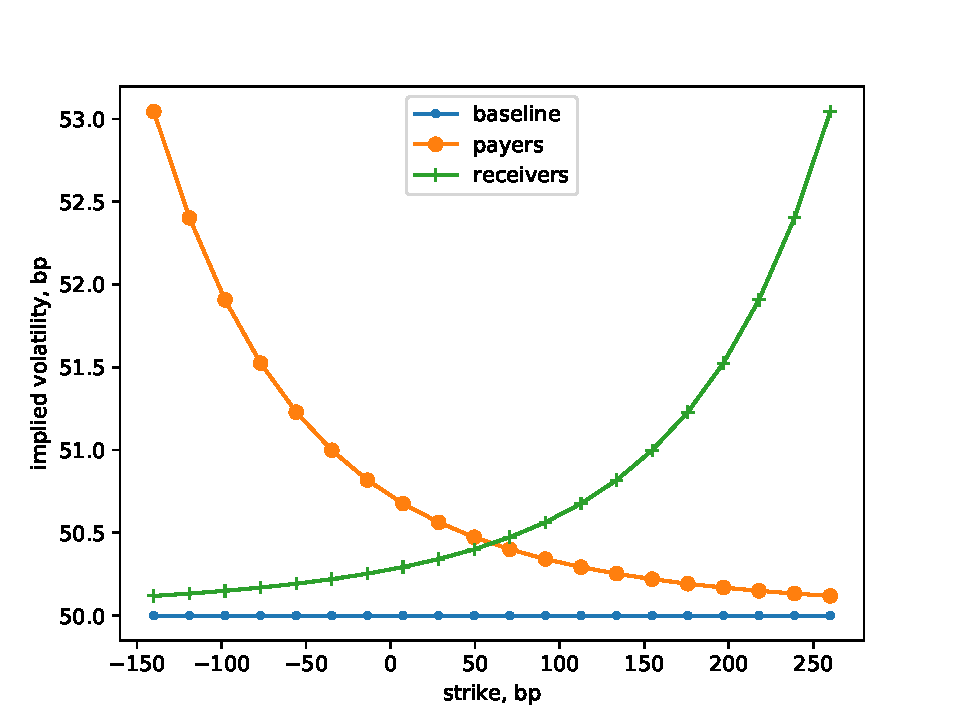
\includegraphics[origin=c,width=0.8\textwidth]{swpt_smile_impact_01.pdf}
\caption{Impact on implied normal volatilities from mismatched discounting.
``Baseline'' is the baseline volatility. ``Payers'' is the volatility
implied from payer swaptions under mismatched discounting. ``Receivers'' is
the volatility implied from receiver swaptions under mismatched discounting.}
\label{fig:swpt_smile_1}
\end{figure}

\section{Caps}

Interest rate caps present another challenge for the benchmark reform, in
this case caused by term Libor rates being replaced by a daily compounded
in-arrears overnight rate, as mentioned in e.g. \cite{henrard-qse1}, \cite%
{henrard-ssrn1}, \cite{risk-fras}.

Let us fix $i$ and simplify notations to $L(t)\triangleq
L_{i}(t)=L(t,T_{i},T_{i}+\tau ),$ $T\triangleq T_{i},$ $\tau \triangleq \tau
_{i}$. The rate $L(t)\ $is given by%
\begin{equation*}
L(t)=\frac{P_{i}(t)-P_{i+1}(t)}{\tau P_{i+1}(t)}.
\end{equation*}%
A caplet is an option that pays $\left( L(T)-K\right) ^{+}$ at time $T+\tau $%
, and its value is given by%
\begin{equation}
V_{\mathrm{LibCpl}}(t)=P(t,T+\tau )\mathrm{E}_{t}^{T+\tau }\left(
L(T)-K\right) ^{+}.  \label{eq:cpl1}
\end{equation}

Under the standard fallback mechanism, a Libor rate would be replaced by a
compounded in-arrears daily rate with a spread, with the payoff in (\ref%
{eq:cpl1}) becoming%
\begin{equation}
V_{\mathrm{OisCpl}}(t)=P(t,T+\tau )\mathrm{E}_{t}^{T+\tau }\left( \frac{1}{%
\tau }\left( \exp \left( \int_{T}^{T+\tau }r(s)~ds\right) -1\right)
-K^{\prime }\right) ^{+},  \label{eq:cpl2}
\end{equation}%
where we use $r(s)$ for the overnight rate, $K^{\prime }$ for the
fallback-spread-adjusted strike, and replace discrete daily with continuous
compounding for notational simplicity.

The fundamental difference between (\ref{eq:cpl1}) and (\ref{eq:cpl2}), as
noted in \cite{henrard-ssrn1}, is that in the former the rate is fixed at
time $T$, whereas in the latter it continues to stochastically evolve until
a later time $T+\tau ,$ combined with the averaging feature of rates fixed
at different times over the time period $[T,T+\tau ].$ A simple European
option in (\ref{eq:cpl1}) becomes an Asian option in (\ref{eq:cpl2}).

Assume for a moment that one-period swaptions are traded. Their value in the
Libor world are given by%
\begin{equation}
V_{\mathrm{LibSwpt}}(t)=P(t,T+\tau )\mathrm{E}_{t}^{T+\tau }\left( V_{%
\mathrm{LibSwap}}(T)\right) ^{+},  \label{eq:cpl3}
\end{equation}%
where%
\begin{equation}
V_{\mathrm{LibSwap}}(T)=\mathrm{E}_{T}^{T+\tau }\left( L(T)-K\right) =L(T)-K.
\label{eq:cpl4}
\end{equation}%
Clearly (\ref{eq:cpl3})--(\ref{eq:cpl4}) describe a contract equivalent to (%
\ref{eq:cpl1}), and in the Libor world a caplet is equivalent to a
one-period swaption. In the post-Libor situation we have%
\begin{equation}
V_{\mathrm{OisSwpt}}(t)=P(t,T+\tau )\mathrm{E}_{t}^{T+\tau }\left( V_{%
\mathrm{OisSwap}}(T)\right) ^{+}  \label{eq:cpl5}
\end{equation}%
with%
\begin{multline}
V_{\mathrm{OisSwap}}(T)=\mathrm{E}_{T}^{T+\tau }\left( \frac{1}{\tau }\left(
\exp \left( \int_{T}^{T+\tau }r(s)~ds\right) -1\right) -K^{\prime }\right) 
\label{eq:cpl6} \\
\neq \frac{1}{\tau }\left( \exp \left( \int_{T}^{T+\tau }r(s)~ds\right)
-1\right) -K^{\prime }.
\end{multline}%
In fact, combining (\ref{eq:cpl5}) and (\ref{eq:cpl6}) we obtain%
\begin{multline}
V_{\mathrm{OisSwpt}}(t)  \label{eq:cpl7} \\
=P(t,T+\tau )\mathrm{E}_{t}^{T+\tau }\left( \mathrm{E}_{T}^{T+\tau }\left( 
\frac{1}{\tau }\left( \exp \left( \int_{T}^{T+\tau }r(s)~ds\right) -1\right)
\right) -K^{\prime }\right) ^{+}.
\end{multline}%
In contrast to (\ref{eq:cpl2}), part of the expectation value operator moves
inside the $\max (\cdot ,0)$ operator. Jensen's inequality (as also noted in 
\cite{lyas-merc-l}) implies%
\begin{equation}
V_{\mathrm{OisCpl}}(t)>V_{\mathrm{OisSwpt}}(t).  \label{eq:cpl8}
\end{equation}

Let us denote 
\begin{equation}
R(t)\triangleq R(t,T,T+\tau )=\mathrm{E}_{t}^{T+\tau }\left( \frac{1}{\tau }%
\left( \exp \left( \int_{T}^{T+\tau }r(s)~ds\right) -1\right) \right) ,
\label{eq:termois1}
\end{equation}%
where $t\in \lbrack 0,T+\tau ]$, i.e.~$t$ is allowed to be larger than $T$
(as in \cite{lyas-merc-l}). For $t\leq T$ this is called the forward term
one-period compounded OIS swap rate and is defined as the break-even rate on
a one-period forward starting OIS swap observed at time $t.$ With this
notation we have%
\begin{equation*}
V_{\mathrm{OisSwap}}(T)=\mathrm{E}_{T}^{T+\tau }\left( R(T)-K^{\prime
}\right)
\end{equation*}%
which is the equivalent of (\ref{eq:cpl4}) in post-Libor world. We note that
the caplet value (\ref{eq:cpl2}) is then%
\begin{equation*}
V_{\mathrm{OisCpl}}(t)=P(t,T+\tau )\mathrm{E}_{t}^{T+\tau }\left( R(T+\tau
)-K^{\prime }\right) ^{+}.
\end{equation*}

\subsection{Market Impact}

A standard interest rate swap post Libor transition looks essentially like a
swap before transition as far as interest rate risk is concerned. Caps,
however, change their character significantly, and may no longer be suitable
for market participants who have them on the books as, for example, a loan
hedge. Sensitivity to volatility looks different, and the complexity of
valuation is different as well, potentially affecting liquidity and the
ability to exit positions.

There is also, of course, the issue of value transfer. A cap versus a
matching tenor swaption, for example a one-year forward starting cap on
three-month Libor versus a one-year swaption with a matching first expiry,
was at times a popular hedge fund trade. Originally designed as a bet on
Libor/swap rate correlations, under the fallback protocol not only will it
likely change its value, but will also acquire different risk
characteristics. A similar divergence may occur between caplets and
exchange-traded options on Eurodollar futures.

\subsection{Volatility Adjustment}

Let us estimate the difference in value of a caplet vs.~a matching
single-period swaption in the post-Libor world. For a very simple estimate,
let us assume that $r(t)$ follows a Brownian motion with constant volatility 
$\sigma $, and let us approximate%
\begin{equation}
R(T+\tau )=\frac{1}{\tau }\left( \exp \left( \int_{T}^{T+\tau
}r(s)~ds\right) -1\right) \approx \widetilde{R}(T+\tau )=\frac{1}{\tau }%
\int_{T}^{T+\tau }r(s)~ds.  \label{eq:va1}
\end{equation}%
To estimate the variance of $\widetilde{R}(T+\tau ),$ we recall (see \cite%
{vp-br}) that for the standard Brownian motion $W(\cdot )$ for $T\geq 0$%
\begin{equation*}
\mathrm{E}\left( \left( \int_{T}^{T+\tau }W(s)~ds\right) ^{2}\right) =\tau
^{2}\left( T+\frac{\tau }{3}\right) .
\end{equation*}%
Thus $\mathrm{Var}\left( \widetilde{R}(T+\tau )\right) =\sigma ^{2}(T+\tau
/3).$ At the same time $\widetilde{R}(T)=r(T)$ under the Brownian motion
assumption and the approximation (\ref{eq:va1}), so that $\mathrm{Var}\left( 
\widetilde{R}(T)\right) =\sigma ^{2}T.$ The ratio of volatilities is then
given by%
\begin{equation}
\frac{\mathrm{Vol}\left( R(T+\tau )\right) }{\mathrm{Vol}\left( R(T)\right) }%
\approx \frac{\mathrm{Vol}\left( \widetilde{R}(T+\tau )\right) }{\mathrm{Vol}%
\left( \widetilde{R}(T)\right) }=\sqrt{1+\frac{\tau }{3T}}  \label{eq:cpl9}
\end{equation}%
(see also \cite{lyas-merk-ssrn}). It is always larger than $1$ as already
discussed, and could be significantly larger than $1$ for shorter-dated
options i.e.~smaller $T.$

\subsection{Skew Adjustment\label{sec:asian_skew}}

The impact of rate averaging on volatility is likely to be the dominant
effect for the volatility smile, but ultimately it is also important to
quantify how averaging affects other smile parameters. We leave the full
treatment of this question for future research, but consider a simple
example here to highlight the magnitude of the likely impact, and to also
introduce a novel quantitative technique for dealing with averaged rates
that is likely to be important in the post-Libor world.

We simplify (\ref{eq:va1}) further by using the trapezoidal rule as in%
\begin{equation*}
\widetilde{R}(T+\tau )\approx \widehat{R}(T+\tau ),\quad \widehat{R}(t)=%
\mathrm{E}_{t}\left( w_{1}r(T_{1})+w_{2}r(T_{2})\right) ,
\end{equation*}%
where $T_{1}=T$, $T_{2}=T+\tau $, and $w_{1}=w_{2}=0.5$ for the trapezoidal
rule, but are left generic with the requirement that $w_{1}+w_{2}=1$ for now.

We define the skew for the set of options on $\widehat{R}(T+\tau
)=w_{1}r(T_{1})+w_{2}r(T_{2})$ as $\overline{\beta }$ in the
shifted-lognormal process%
\begin{equation*}
dY(t)=\overline{\lambda }(\overline{\beta }Y(t)+(1-\overline{\beta })%
\widehat{R}_{0})~d\overline{W}(t),\quad \widehat{R}_{0}=\widehat{R}(0),
\end{equation*}%
such that 
\begin{equation}
\mathrm{E}\left( Y(T)-K\right) ^{+}\approx \mathrm{E}\left( \widehat{R}%
(T+\tau )-K\right) ^{+}=\mathrm{E}\left(
w_{1}r(T_{1})+w_{2}r(T_{2})-K\right) ^{+}\text{ }\forall K.  \label{eq:sa1}
\end{equation}%
For inspiration we recall the derivation of the basket skew from \cite%
{ant-mis}, as covered in \cite[Section A.4]{ap-book}. The options on the
right-hand side of (\ref{eq:sa1}) look like options on a basket except the
underlying(s) are observed at different times. We deal with this
complication via time change, a technique that we believe can be generally
applied to derive other volatility parameters for options on time\ averages.
We define%
\begin{equation*}
X_{1}(t)=r(t),\quad X_{2}(t)=r(tT_{2}/T_{1}),
\end{equation*}%
so that the right-hand side of (\ref{eq:sa1}) is given by%
\begin{equation*}
\mathrm{E}\left( w_{1}X_{1}(T)+w_{2}X_{2}(T)-K\right) ^{+},
\end{equation*}%
which now looks indeed like a basket option and \cite[Section A.4]{ap-book}
can be applied. Assuming shifted-lognormal process for the overnight rate%
\begin{equation*}
dr(t)=\sigma (\beta r(t)+(1-\beta )r_{0})~dW(t),
\end{equation*}%
time-change calculations lead to%
\begin{equation*}
dX_{i}(t)=\sigma _{i}(\beta X_{i}(t)+(1-\beta )r_{0})~dW_{i}(t),\quad i=1,2,
\end{equation*}%
where%
\begin{equation*}
\sigma _{1}=\sigma ,\quad \sigma _{2}=\left( T_{2}/T_{1}\right) ^{1/2}\sigma
,\quad W_{1}(t)=W(t),\quad W_{2}(t)=\left( T_{1}/T_{2}\right)
^{1/2}W(tT_{2}/T_{1}),
\end{equation*}%
and%
\begin{equation*}
\rho \triangleq \mathrm{corr}(W_{1}(t),W_{2}(t))=\left( T_{1}/T_{2}\right)
^{1/2}.
\end{equation*}%
Applying \cite[Proposition A.4.1]{ap-book} we obtain, after some
manipulations, that%
\begin{equation}
\overline{\beta }=\beta \frac{w_{1}\left( w_{1}+w_{2}\right)
^{2}+w_{2}\left( w_{1}+w_{2}\left( T_{2}/T_{1}\right) \right) ^{2}}{\left(
w_{1}^{2}+2w_{1}w_{2}+w_{2}^{2}\left( T_{2}/T_{1}\right) \right) ^{2}},
\label{eq:sa2}
\end{equation}%
which is our main result for the skew of (the discrete approximation to)\ an
Asian option. For $w_{1}=1$ ($w_{2}=0$) or $w_{1}=0$ ($w_{2}=1$) we
naturally obtain $\overline{\beta }=\beta ,$ and for $w_{1}=w_{2}=0.5$ we
obtain%
\begin{equation*}
\overline{\beta }=\beta \frac{10+4\left( T_{2}/T_{1}\right) +2\left(
T_{2}/T_{1}\right) ^{2}}{9+6\left( T_{2}/T_{1}\right) +\left(
T_{2}/T_{1}\right) ^{2}}.
\end{equation*}%
Specifically, for $T_{2}/T_{1}=2$ (e.g.~$T=1$, $\tau =1$),%
\begin{equation*}
\overline{\beta }=\frac{26}{25}\beta =1.04b,
\end{equation*}%
so the skew is adjusted by $4\%$ relative. While not large, it is
noticeable, as we show in Figure~\ref{fig:asian_skew_1}, where we also
demonstrate the quality of our approximation. For $T_{2}/T_{1}=10,$ the the
case of a rather short expiry, $\overline{\beta }\approx 1.48b,$ i.e. almost 
$50\%$ relative adjustment to the skew.

\begin{figure}[ht]
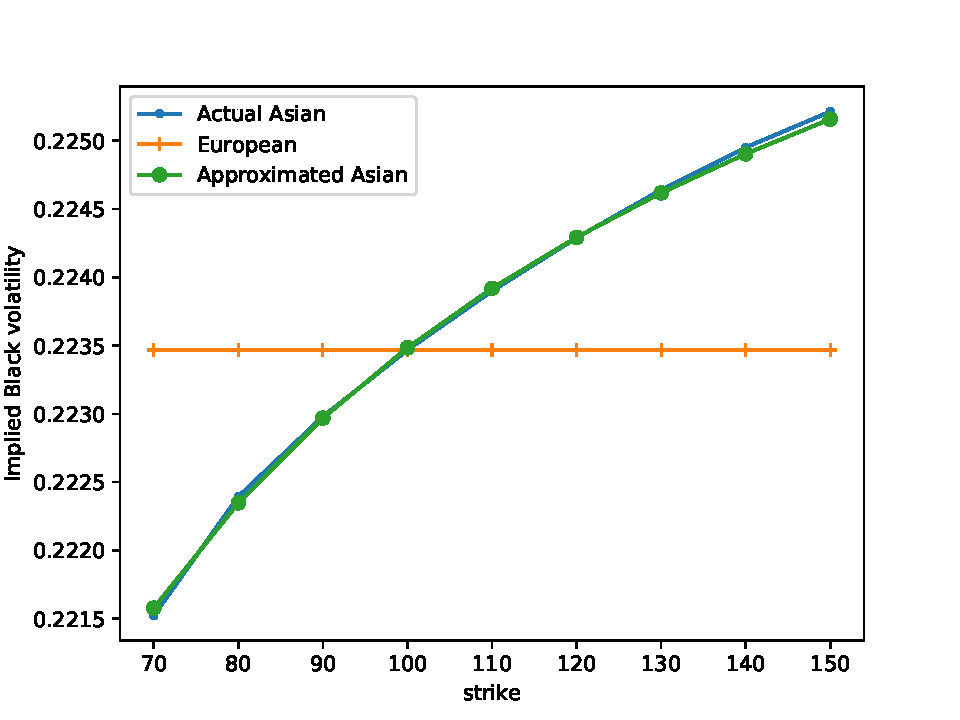
\includegraphics[origin=c,width=0.8%
\textwidth]{fig_skew_appr_vs_actual_01.pdf}
\caption{Asian (two-element basket) option skew approximation from Section~%
\protect\ref{sec:asian_skew}. Overnight rate $r(\cdot)$ follows a
shifted-lognormal process with spot $100$, volatility $20$\% and skew $100$%
\%. Weights $w_1=w_2=0.5$. $T=1$, $\protect\tau=1$. ``Actual'' is calculated
by a numerical scheme. ``European'' uses $100$\% skew. ``Approximated
Asian'' uses our approximation.}
\label{fig:asian_skew_1}
\end{figure}

\subsection{Considerations for Modelling}

Modeling caps post-Libor transition is more complicated as the option
becomes Asian. In this regard, \cite{henrard-ssrn1} derives valuation
formulas in a one-factor Gaussian model, and of course the seminal extension
of the Libor market model for overnight rates from \cite{lyas-merc-l} can be
used. Both, however, are likely to be deemed impractical by traders for what
would still be likely considered a vanilla product. Hence, an adaptation of
a vanilla model such as SABR will likely be required.

It is possible that both types of contracts, Asian-style OIS caplets and
European style single-period swaptions, will be traded in the future. This
possibility should be one of the considerations of any future vanilla risk
management framework. In particular the model should be flexible enough so
that the two types of contracts can be marked at different levels of
volatility and, potentially, of other volatility smile parameters. In
particular, it seems unlikely that a simple scaling of swaption volatility
along the lines of (\ref{eq:cpl9}), or skew as in (\ref{eq:sa2}), would be
sufficient to match both markets.

The relations (\ref{eq:cpl9}), (\ref{eq:sa2}) do, however, help as they
express volatilities and skews of different contracts in a comparable way.
Let us assume we mark single-period OIS swaptions with expiry $T$ and tenor $%
\tau $ with parameters, in the standard SABR parameterization, $\sigma _{%
\mathrm{swpt}},$ $\alpha _{\mathrm{swpt}},$ $\beta _{\mathrm{swpt}},$ $\rho
_{\mathrm{swpt}}$. It is natural then to use a SABR model for caplets as
well. We would then mark $\sigma _{\mathrm{cpl}},$ $\beta _{\mathrm{cpl}}$
as we see fit and, perhaps, in the first iteration of the model use the same
values for other parameters, $\alpha _{\mathrm{cpl}}=\alpha _{\mathrm{swpt}%
}, $ $\rho _{\mathrm{cpl}}=\rho _{\mathrm{swpt}}.$ Before applying the SABR
model to a caplet we would first transform $\sigma _{\mathrm{cpl}},$ $\beta
_{\mathrm{cpl}}$ into an approximation to the \textquotedblleft Asian
volatility and skew\textquotedblright\ using (\ref{eq:cpl9}), (\ref{eq:sa2})
by setting%
\begin{equation}
\sigma _{\mathrm{asian}}=\sigma _{\mathrm{cpl}}\sqrt{1+\tau /(3T)},\quad
\beta _{\mathrm{asian}}=\beta _{\mathrm{cpl}}\frac{10+4\left( 1+\tau
/T\right) +2\left( 1+\tau /T\right) ^{2}}{9+6\left( 1+\tau /T\right) +\left(
1+\tau /T\right) ^{2}}  \label{eq:cpl10}
\end{equation}%
for $T\geq 0$. We would use the set of parameters 
\begin{equation*}
\sigma _{\mathrm{asian}},\alpha _{\mathrm{cpl}},\beta _{\mathrm{asian}},\rho
_{\mathrm{cpl}}
\end{equation*}%
in the SABR formula to calculate (\ref{eq:cpl2}) with the strike $K^{\prime
} $ and the forward set to $R(0)$ (or the exact daily compounding version
thereof). The scalings (\ref{eq:cpl10}), while not strictly necessary,
express caplets versus swaptions, and caplets of different expiries, in
normalized units and thus help in hedging and marking activities.

\section{Disappearing Species?}

Interest rate caps change quite significantly under the standard Libor
fallback. Some of the other products may be affected even more and disappear
altogether.

\subsection{Libor-In-Arrears}

In a Libor-In-Arrears (LIA, see \cite{ap-book}) swap, the floating leg pays
a Libor rate as soon as it is fixed. The fallback for Libor, the in-arrears
compounded overnight rate, works well for a standard swap but not for an
in-arrears swap as the fallback rate will simply not be known at the
beginning of the accrual period. So while caps get transformed into
meaningful, although different from the original, contracts, LIA swaps
simply do not work under the standard fallback, similar to FRAs (see \cite%
{henrard-qse1}). Let us look at how this issue could be prevented by
modifying LIA swaps accordingly.

Clearly a term version of the risk-free rate -- a fixed break-even rate one
would pay on a one-period swap against the compounded in-arrears overnight
rate such as (\ref{eq:termois1}) -- would be a near perfect substitute for a
Libor rate in an LIA swap, as well as for many other Libor-linked contracts
such as FRAs. Regulators so far have discouraged reliance on the potential
existence of such rates for derivatives fallback. So let us consider what
can be done with overnight compounded rates. The prevailing commercial
rationale for customers to trade LIA, rather than standard, swaps is that on
a receiver swap the client would pay Libor-based payments sooner than in a
normal swap, and also the dealer would benefit from LIA convexity, so he
would pay a higher fixed rate.

Libor rate $L(t)=L(t,T,T+\tau ),$ if paid in-arrears, is worth at time $t$
(see \cite{ap-book})%
\begin{equation*}
V_{\mathrm{LibLis}}(t)=P(0,T)\mathrm{E}_{t}^{T}L(T)=P(0,T+\tau )\mathrm{E}%
_{t}^{T+\tau }\left( L(T)\left( 1+\tau L(T)\right) \right) .
\end{equation*}%
A payment of Libor at time $T$ is financially equivalent to a payment of
\linebreak $L(T)\left( 1+\tau L(T)\right) $ at time $T+\tau .$ The latter is
much more amendable to the proposed standard fallback, and we can simply
replace a LIA swap with a contract that pays $\tilde{R}(1+\tau \tilde{R})$
at time $T+\tau ,$ where $\tilde{R}=R(T+\tau )+F$ as defined by (\ref%
{eq:termois1}), with $F$ being the fallback spread. Note that a similar fix
works for an FRA. It is fair to note that while this fix is theoretically
\textquotedblleft perfect\textquotedblright , operational considerations
such as payment timings and the need to change underlying legal
documentation may make this approach not practically feasible (see also ).

\subsection{Range Accruals}

Things get more complicated still with range accruals, a popular Libor
exotic often embedded in structured notes, sometimes in callable form (see 
\cite{ap-book}). A basic range accrual (RA) coupon pays 
\begin{equation}
\int_{T}^{T+\delta }1_{\{L_{0}(t)>a\}}dt  \label{eq:RA1}
\end{equation}%
at time $T+\delta ,$ where $L_{0}(t)\triangleq L(t,t,t+\tau )$ is the
current time-$t$ (signified by the subscript $0$) Libor fixing, and $a$ is a
lower barrier. As with LIA, a direct replacement of $L_{0}(t)$ with the
standard fallback compounded overnight rate does not work as it is not known
at time $t$, and hence the payment cannot be made at $T+\delta .$ Let us see
what happens if we directly replace $L_{0}(t)$ in (\ref{eq:RA1}) with $%
R_{0}(t)\triangleq R(t+\tau ,t,t+\tau ),$ where the subscript $0$ signifies
that the rate starts compounding immediately on the observation date.
Ignoring the adjustment of the barrier $a$ for the Libor-OIS fallback
spread, the payoff becomes%
\begin{equation*}
\int_{T}^{T+\delta }1_{\{R_{0}(t)>a\}}dt,
\end{equation*}%
and is fully known only at time $T+\delta +\tau ,$ and not at time $T+\delta 
$ for the original contract. Therefore it cannot be paid earlier than $%
T+\delta +\tau $; to preserve the economics of discounting we can compound
it by the rate from $T+\delta $ to $T+\delta +\tau $, thus replacing (\ref%
{eq:RA1}) with%
\begin{equation}
\left( 1+\tau R_{0}\left( T+\delta \right) \right) \int_{T}^{T+\delta
}1_{\{R_{0}(t)>a\}}dt  \label{eq:RA2}
\end{equation}%
paid at $T+\delta +\tau .$

Paying a certain amount on a given date is economically equivalent to paying
a properly un-discounted value at a later date; operationally, however,
these two payments are not the same. For example, an investor in a
structured note with an embedded range accrual rightfully expects coupon and
principal payments on the agreed-upon dates and not on some future dates,
and may be reluctant to accept changes. This is yet another manifestation of
the practical challenges of the benchmark reform implementation for
structured products.

This is not the end of the story, however. The same issue that we had with
Libor caps turning \textquotedblleft Asian\textquotedblright\ under the
fallback is present here as well. Whereas an option that pays $%
1_{\{L_{0}(t)>a\}}$ is a European-style digital option and can be valued
directly from the caplet smile for time $t,$ an option that pays $%
1_{\{R_{0}(t)>a\}}$ is an option on an average rate with the observations
for the average covering the time interval $[t,t+\tau ].$ The underlying
rate will have higher volatility but the impact of that on the digital
option value can be in either direction. Hence, even if we go into the
trouble of restructuring range accrual swaps with clients from paying (\ref%
{eq:RA1}) to (\ref{eq:RA2}), there will still be potentially significant
value transfer and risk impact that would need to be dealt with.

\section{Conclusions}

We explored a number of areas where rates benchmark reform affects
non-linear rates markets in significant ways. While by no means exhaustive,
even the cases we consider demonstrate the sheer amount of further
considerations and work required to bring Libor termination to a successful
conclusion. We have made a number of practical suggestions on how the
biggest challenges could be overcome. It is clear however that replacing
term Libor rates with compounded overnight rates in all possible use cases
in non-linear markets remains a formidable challenge.

\section*{Acknowledgments}

I would like to thank Pierre-Yves Guerber, Phil Lloyd, Oliver Cooke,
Vladimir Golovanov, Oscar Arias, Marc Henrard and Andrei Lyashenko for
thoughtful comments and discussions. Anonymous referees provided very useful
feedback that significantly improved the paper. All remaining errors are
mine.

\section*{Disclaimer}

Opinions expressed in this article are those of its author and do not
necessarily reflect the views and policies of NatWest Markets or any other
organization.

\begin{thebibliography}{99}
\bibitem{ap-book} L.~Andersen and V.~Piterbarg, "`Interest Rate Modelling",
in three volumes, 2010, Atlantic Financial Press

\bibitem{ant-mis} A. Antonov and T. Misirpashaev. "Markovian projection onto
a displaced diffusion: Generic formulas with applications", 12(4):507--522,
2009a, International Journal of Theoretical and Applied Finance

\bibitem{arrc} Alternative Reference Rates Committee, \textquotedblleft ARRC
consultation on swaptions impacted by the CCP discounting transition to
SOFR\textquotedblright , February 2020,
https://www.newyorkfed.org/medialibrary/Microsites/arrc/files/ 2020/
ARRC\_Swaption\_Consultation.pdf

\bibitem{risk-presess} H. Bartholomew, "LCH targets hardwired pre-cessation
triggers", January 2020, Risk.net

\bibitem{risk-bonds} B. St. Clair. "Libor fallbacks a low priority for most
bond investors", March 2019, Risk.net

\bibitem{cme-ds} CME group, ``SOFR discounting \& price alignment transition
plan for cleared USD interest rate swaps'', December 2019,
www.cmegroup.com/education/articles-and-reports/sofr-price-alignment-and-discounting-proposal.html

\bibitem{risk-mh1} M. Henrard, "Signing the Libor fallback protocol: a
cautionary tale", January 2020, Risk.net

\bibitem{henrard-qse1} M. Henrard, "A Quant perspective on LIBOR fallback",
March 2019, Quant Summit Europe conference

\bibitem{henrard-ssrn1} M. Henrard, "A Quant perspective on IBOR fallback
consultation results - V2.1", January 2019, Available at SSRN:
https://ssrn.com/abstract=3308766

\bibitem{lyas-merc-l} A. Lyashenko and F. Mercurio, "Libor replacement: a
modelling framework for in-arrears term rates", November 2019, Risk Magazine

\bibitem{lyas-merk-ssrn} A. Lyashenko and F. Mercurio, "Looking Forward to
Backward-Looking Rates: A Modeling Framework for Term Rates Replacing
LIBOR", February, 2019, Available at SSRN: https://ssrn.com/abstract=3330240

\bibitem{risk-swpt} R. Mackenzie Smith, "LCH won't back single fix for
swaptions", November 2020, Risk.net

\bibitem{po-vp} P. Orgler and V. Piterbarg, \textquotedblleft Does rates
reform for structured notes lack structure?\textquotedblright , April 2020,
Risk.net

\bibitem{vp-disc} V. Piterbarg, "Funding beyond discounting: collateral
agreements and derivatives pricing", February 2010, Risk Magazine, pp.97--102

\bibitem{vp-br} V. Piterbarg, "Interest rates benchmark reform and options
markets", February 2020, Available at SSRN: https://ssrn.com/abstract=3537925

\bibitem{risk-fras} N. Sherif, "FRAs won't work with standard Libor
fallback, experts say", March 2019, Risk.net
\end{thebibliography}

\end{document}
